\section{Architectural Design}
\subsection{Overview}
The figure shown below represents a high-level description of the components which make up the System.
In this document the presentation layer and the Client (e.g. the Browser)
will be referred to as the Frontend, while the Application Layer and the Data Layer
will be referred to as the Backend.

\begin{figure}[H]
    \centering
    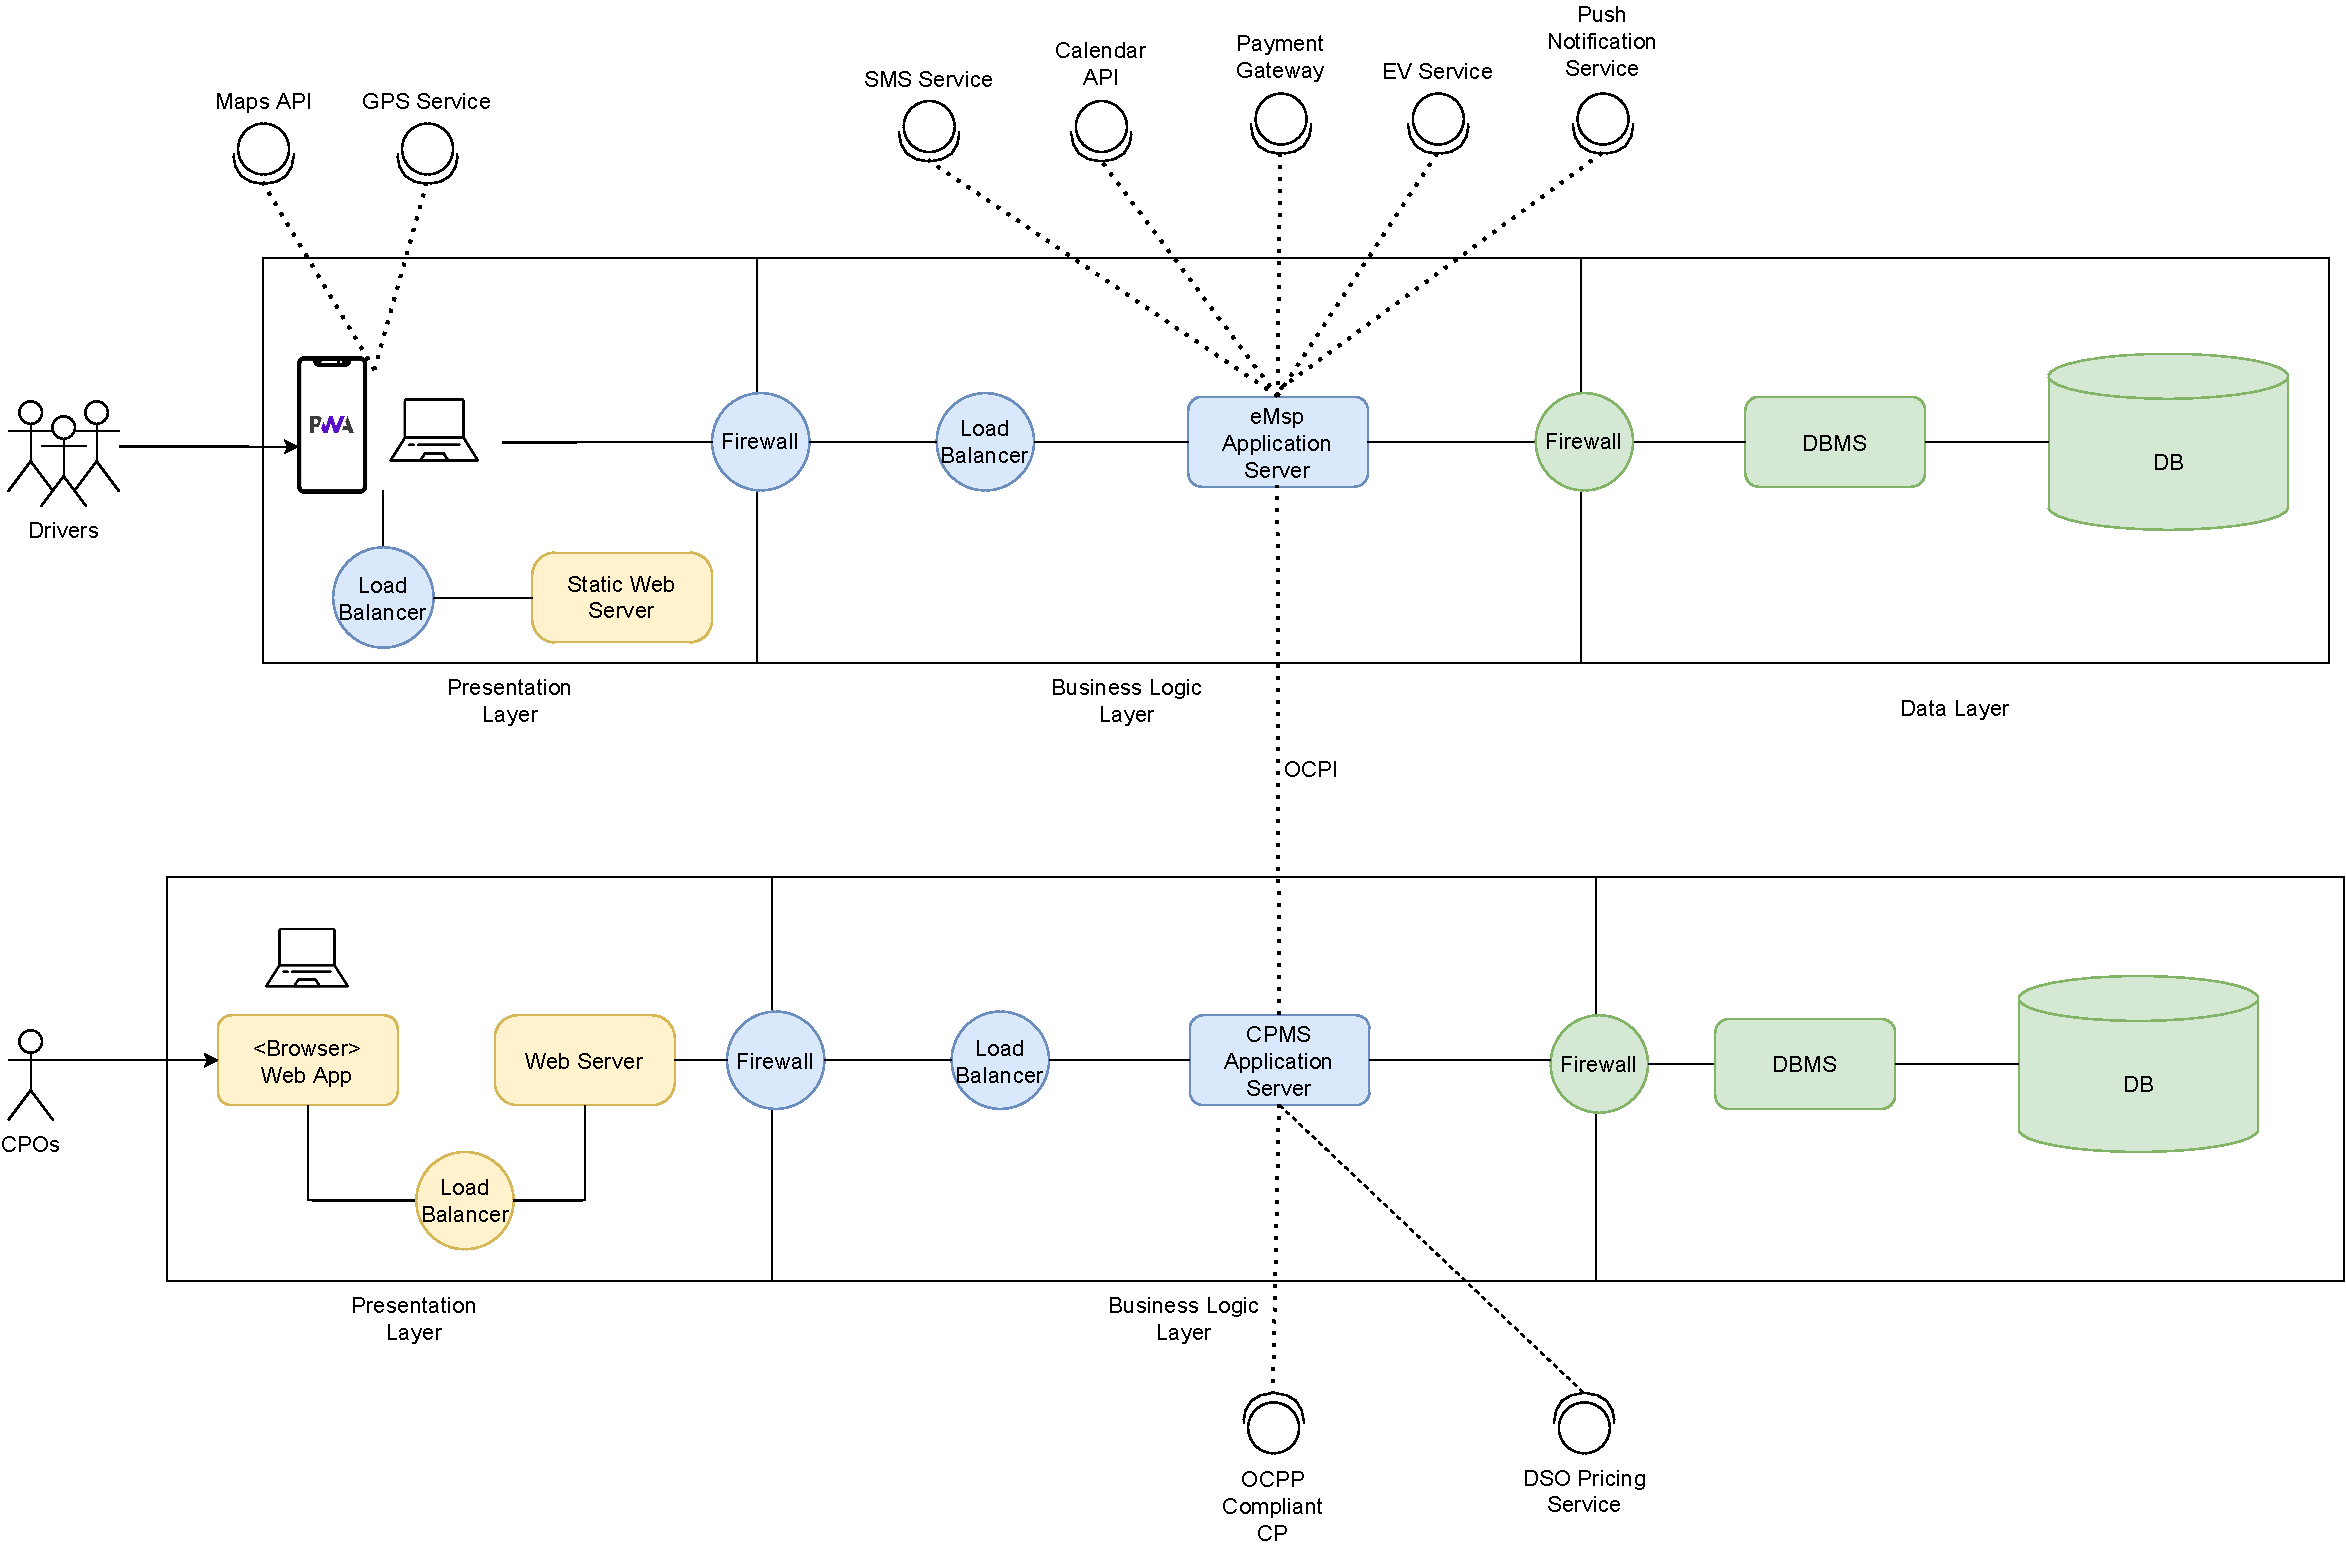
\includegraphics[scale=0.42]{src/Overview/overview_diagram.pdf}
\end{figure}

\hfill \\
The service is supposed to be accessed through a web interface.
For the users, both drivers and CPOs, of the system an SPA will be developed. An SPA is well-suited for applications
that require a lot of interaction and do not need to perform frequent full page reloads.
Furthermore, they can provide a faster and more seamless user experience.
The Overview Architecture of the S2B divides the application in the layers described
above.
The application servers interfaces with the DBMS APIs, in order
to retrieve and store the data required for the considered computation.
The applications servers are expected to be stateless, according to the
REST standard definitions. The nodes are separated by firewalls to guarantee a higher level of security
of the whole system.
\pagebreak
\subsection{Component view}
In this section we show the components of the S2B, their relationships and interfaces. The following sections will explain the interaction between interfaces and details on each method of interfaces with REST endpoints, if any.

\begin{figure}[H]
    \centering
    \hspace*{-2cm}
    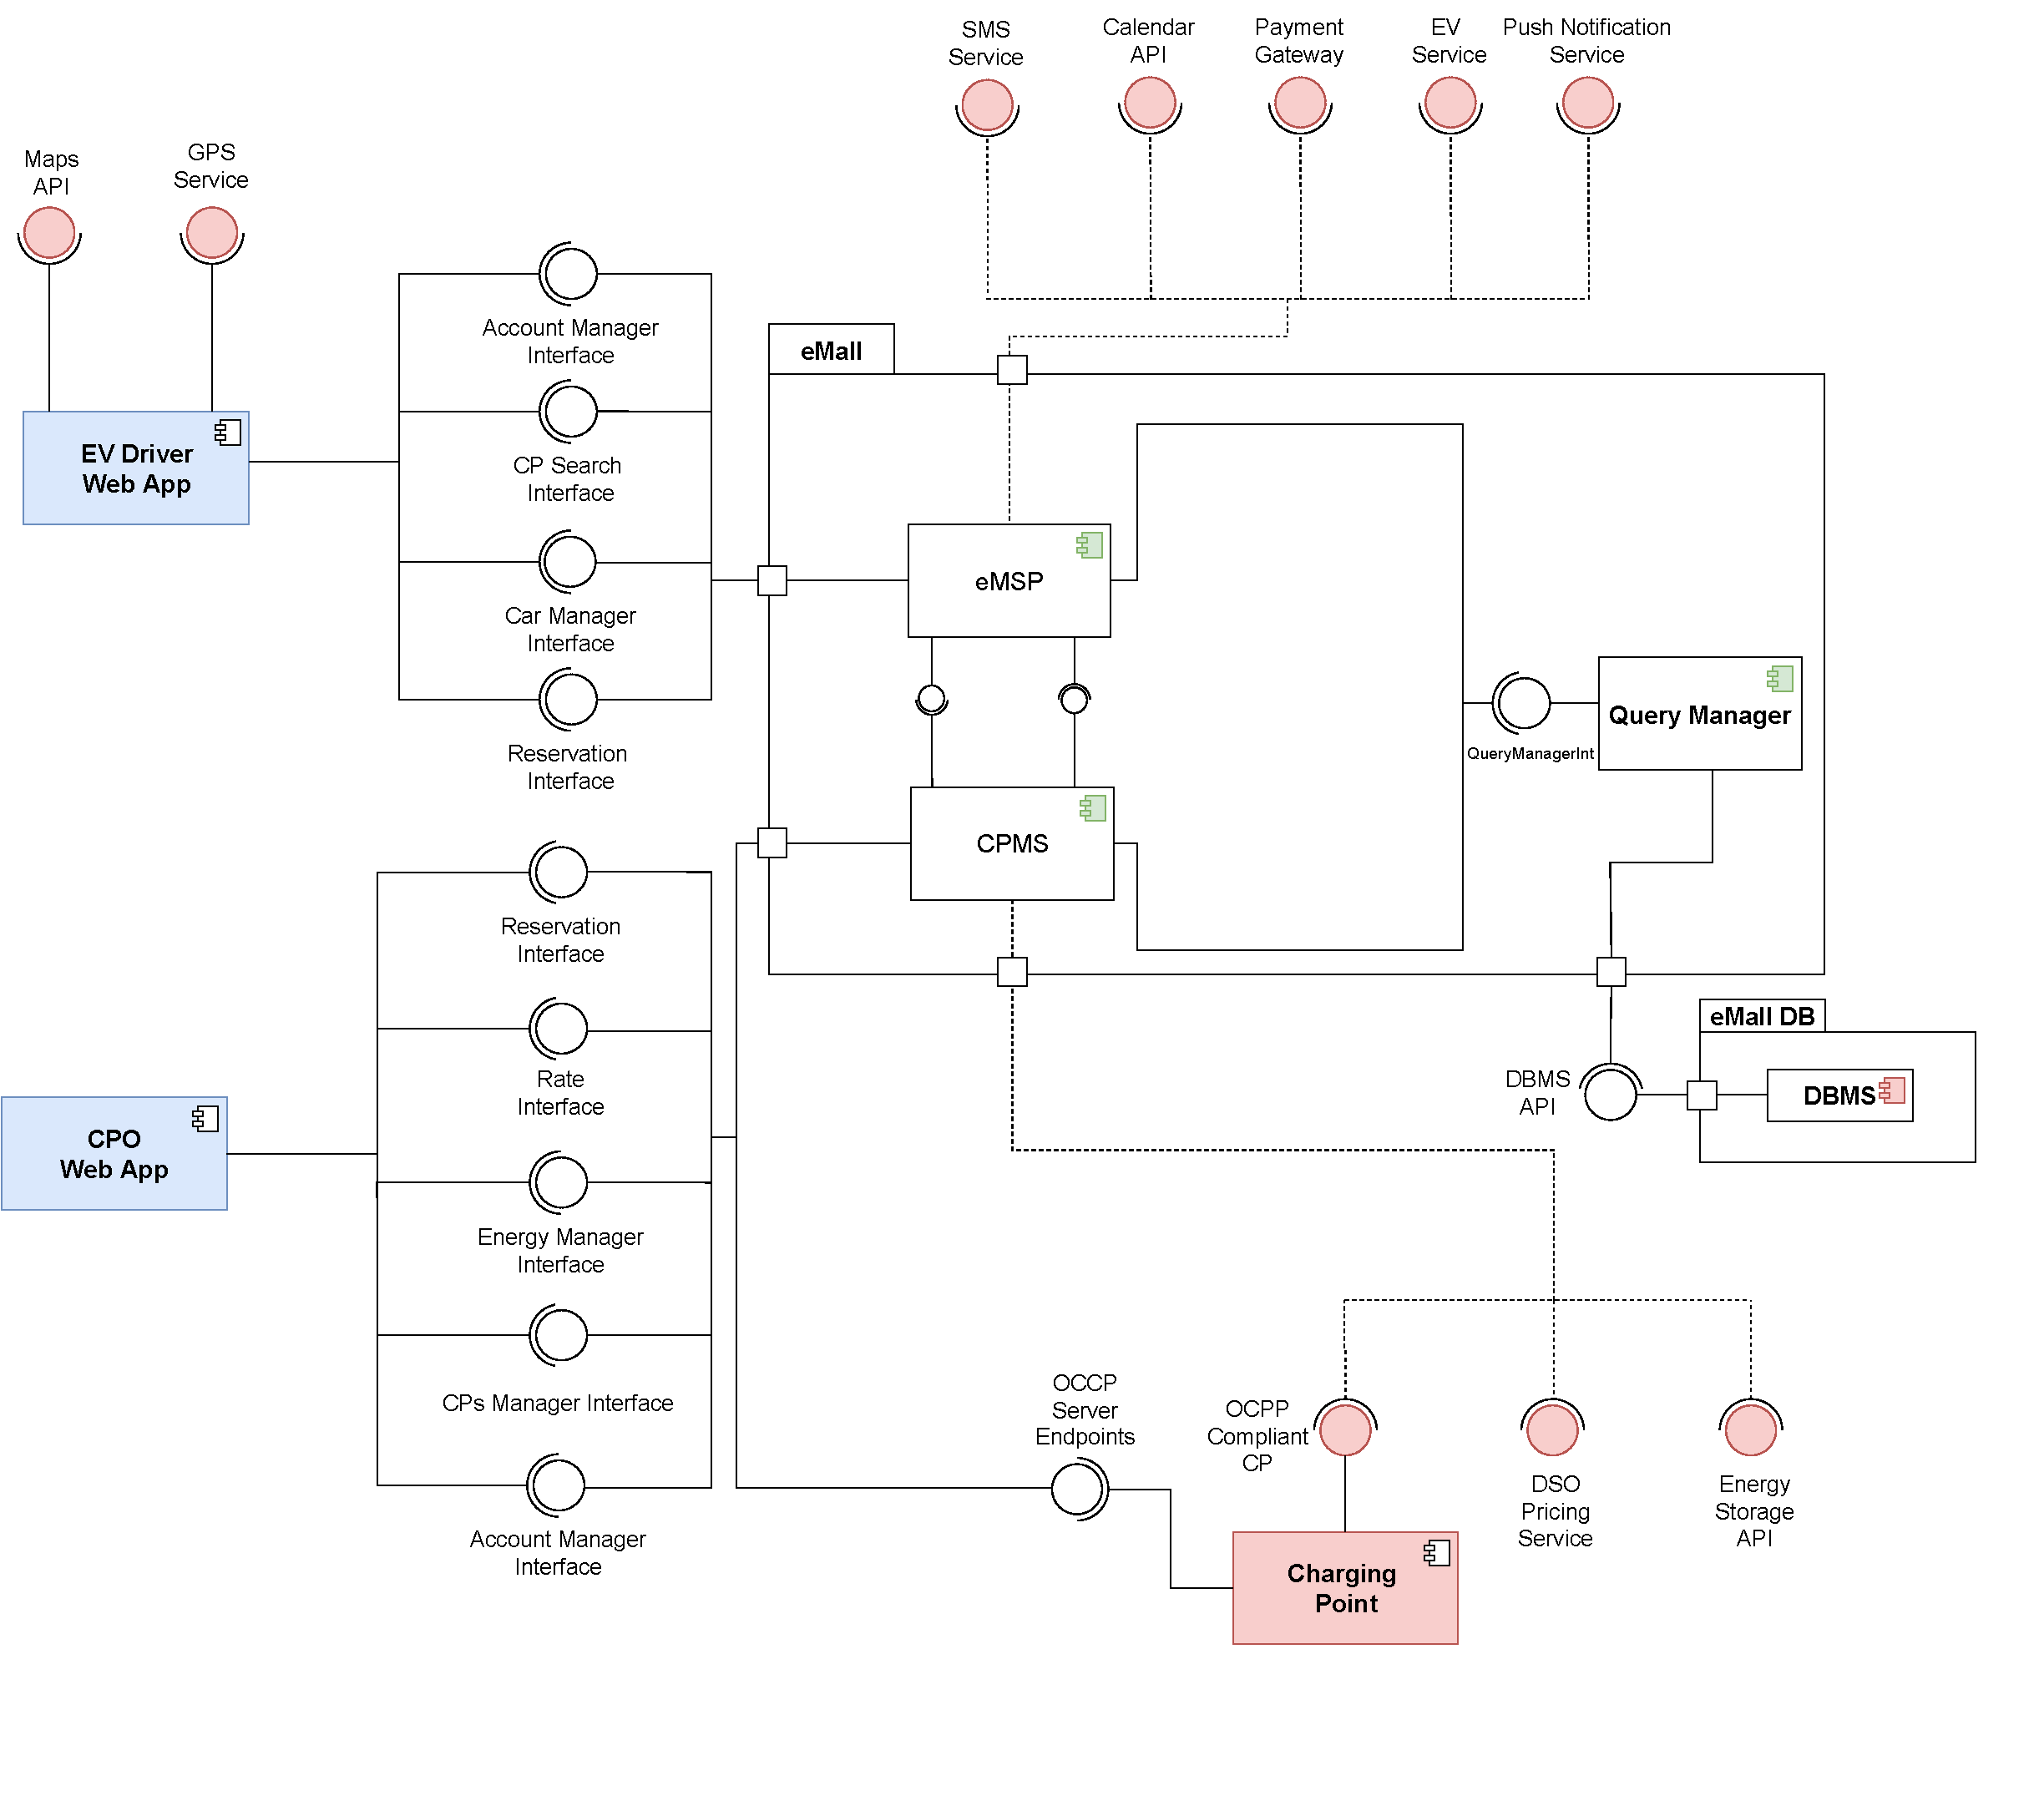
\includegraphics[scale=0.5]{src/ComponentDiagram/overview_component_diagram.pdf}
    \caption{Component Diagram of the eMall System}
\end{figure}


\subsubsection{eMSP}

\begin{figure}[H]
    \centering
    \hspace*{-2cm}
    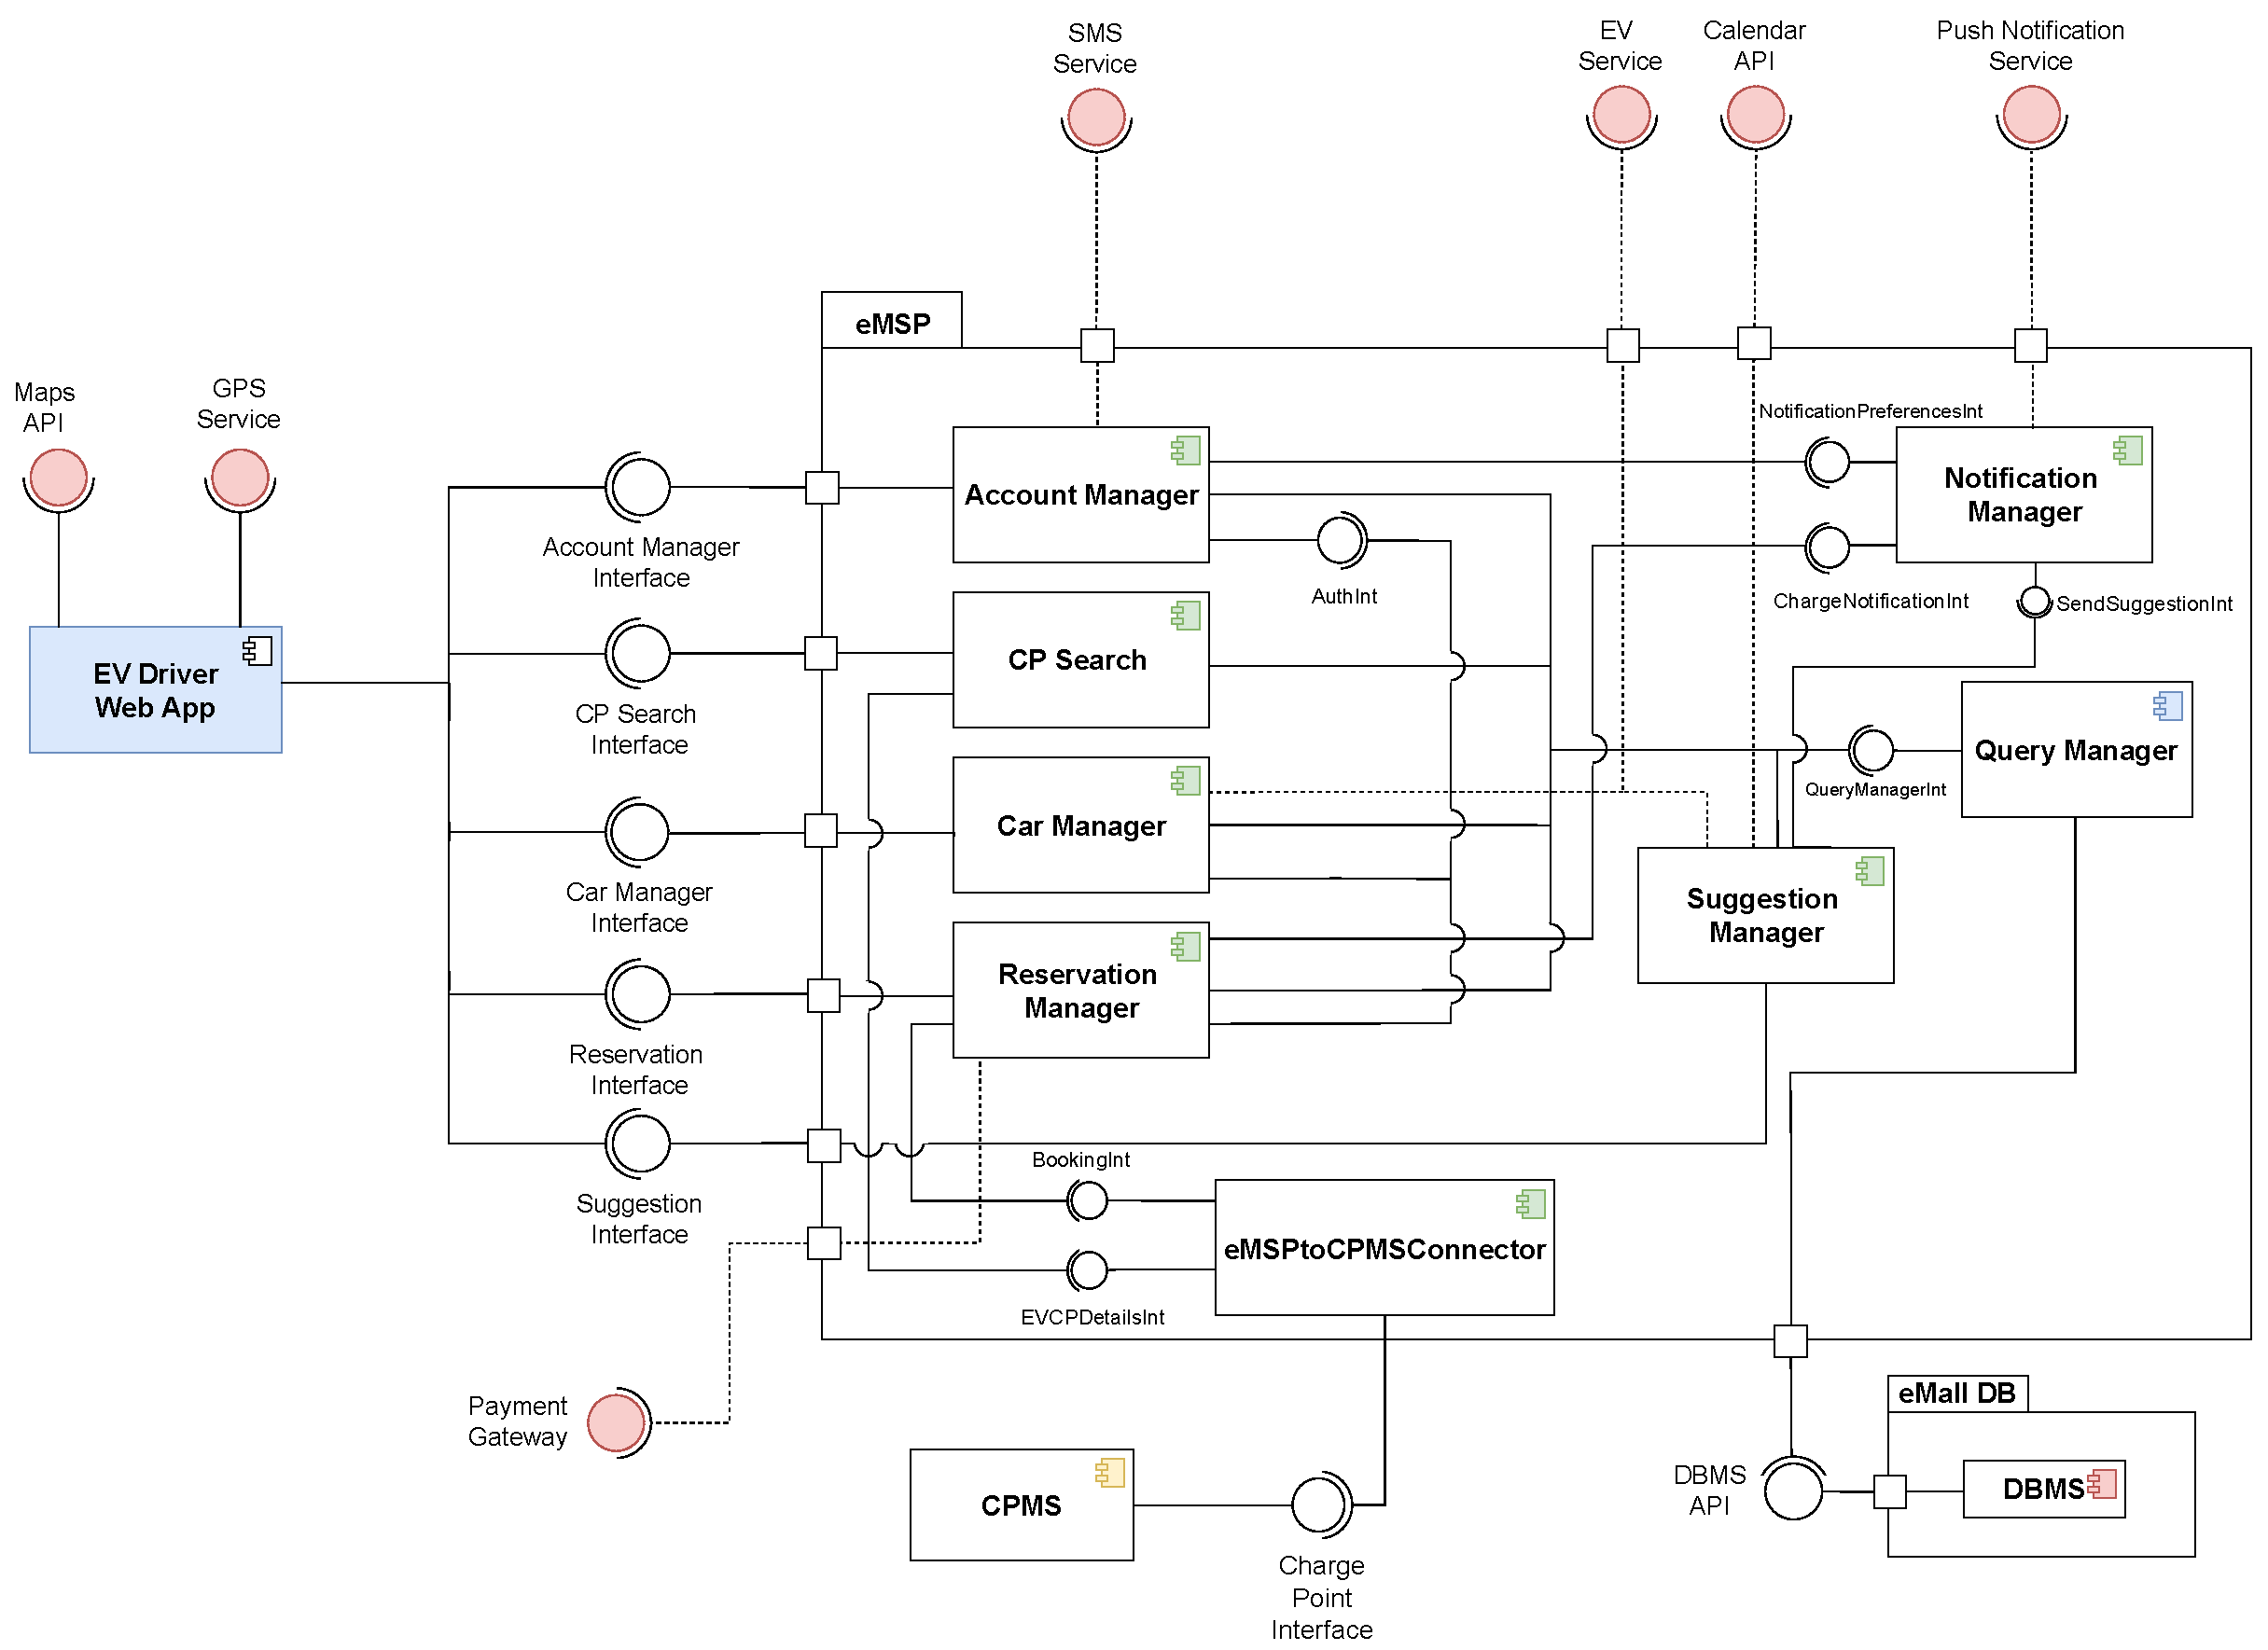
\includegraphics[scale=0.48]{src/ComponentDiagram/emsp_component_diagram.pdf}
    \caption{Component Diagram of the eMSP subsystem}
\end{figure}

\paragraph*{eMSP Web App} \hfill \\
It represents the application dedicated to the EV drivers. This component uses client side rendering of web pages.
The user through the browser sends a request to the server and the eMSP Application Server responds with the HTML and Javascript which the browser then
downloads and execute. As the user interacts with the page, the Javascript can make additional requests to the server and update
the page dynamically, without need to fully reload the page.
\paragraph*{eMSP Application Server} \hfill \\
The eMSP Application Server is responsible for the business logic to provide the functionality to the application for the EV Drivers and to coordinate the information flow between application layer and data layer
It is composed of several components, each of them used for a specific functionality:\\
\begin{itemize}
    \item \textbf{eMPS's Account Manager} \\ This component handles all the account operations related to the CPO and offers an interface to authenticate
          the requests in the CPMS application server.
          It offers functionality to create new account, logging in, setting preferences and verify the authentication of the user at any time.
          To create a new account interacts with the external SMS API to make the user receive a code to verify the identity.
    \item \textbf{CP Search} \\ This component handles the operations needed to show the CPs in a specified range of km near a location. The location
          can be described as an address, with coordinates or by geolocating the actual position of the incoming request. It selects the filtered CPs that are then
          shown in the map as placeholders.
    \item \textbf{Car Manager} \\ This component handles the operations related to the status of the car. It offers an interface to select the EV model among a list of
          all the marketed models and offers an interface to connect the car to the application. It uses these information to show the battery status of the EV, the
          amount of power during a charging process and to suggest charging plans based on the specific vehicle and status of it.
    \item \textbf{Reservation Manager} \\ This component handles all the operations related to the reservations for the EV Drivers. It offers the possibility to create a reservation
          for a charge and pay for that reservation, see the details of a reservation, start or pause a charge of a particular reservation and see the recap of an already occurred reservation.
          It permits to pay for a reservation using an external Payment Gateway that handles all the payment process and returns the status of the payment.

\end{itemize}


\subsubsection{CPMS}

\begin{figure}[H]
    \centering
    \hspace*{-2cm}
    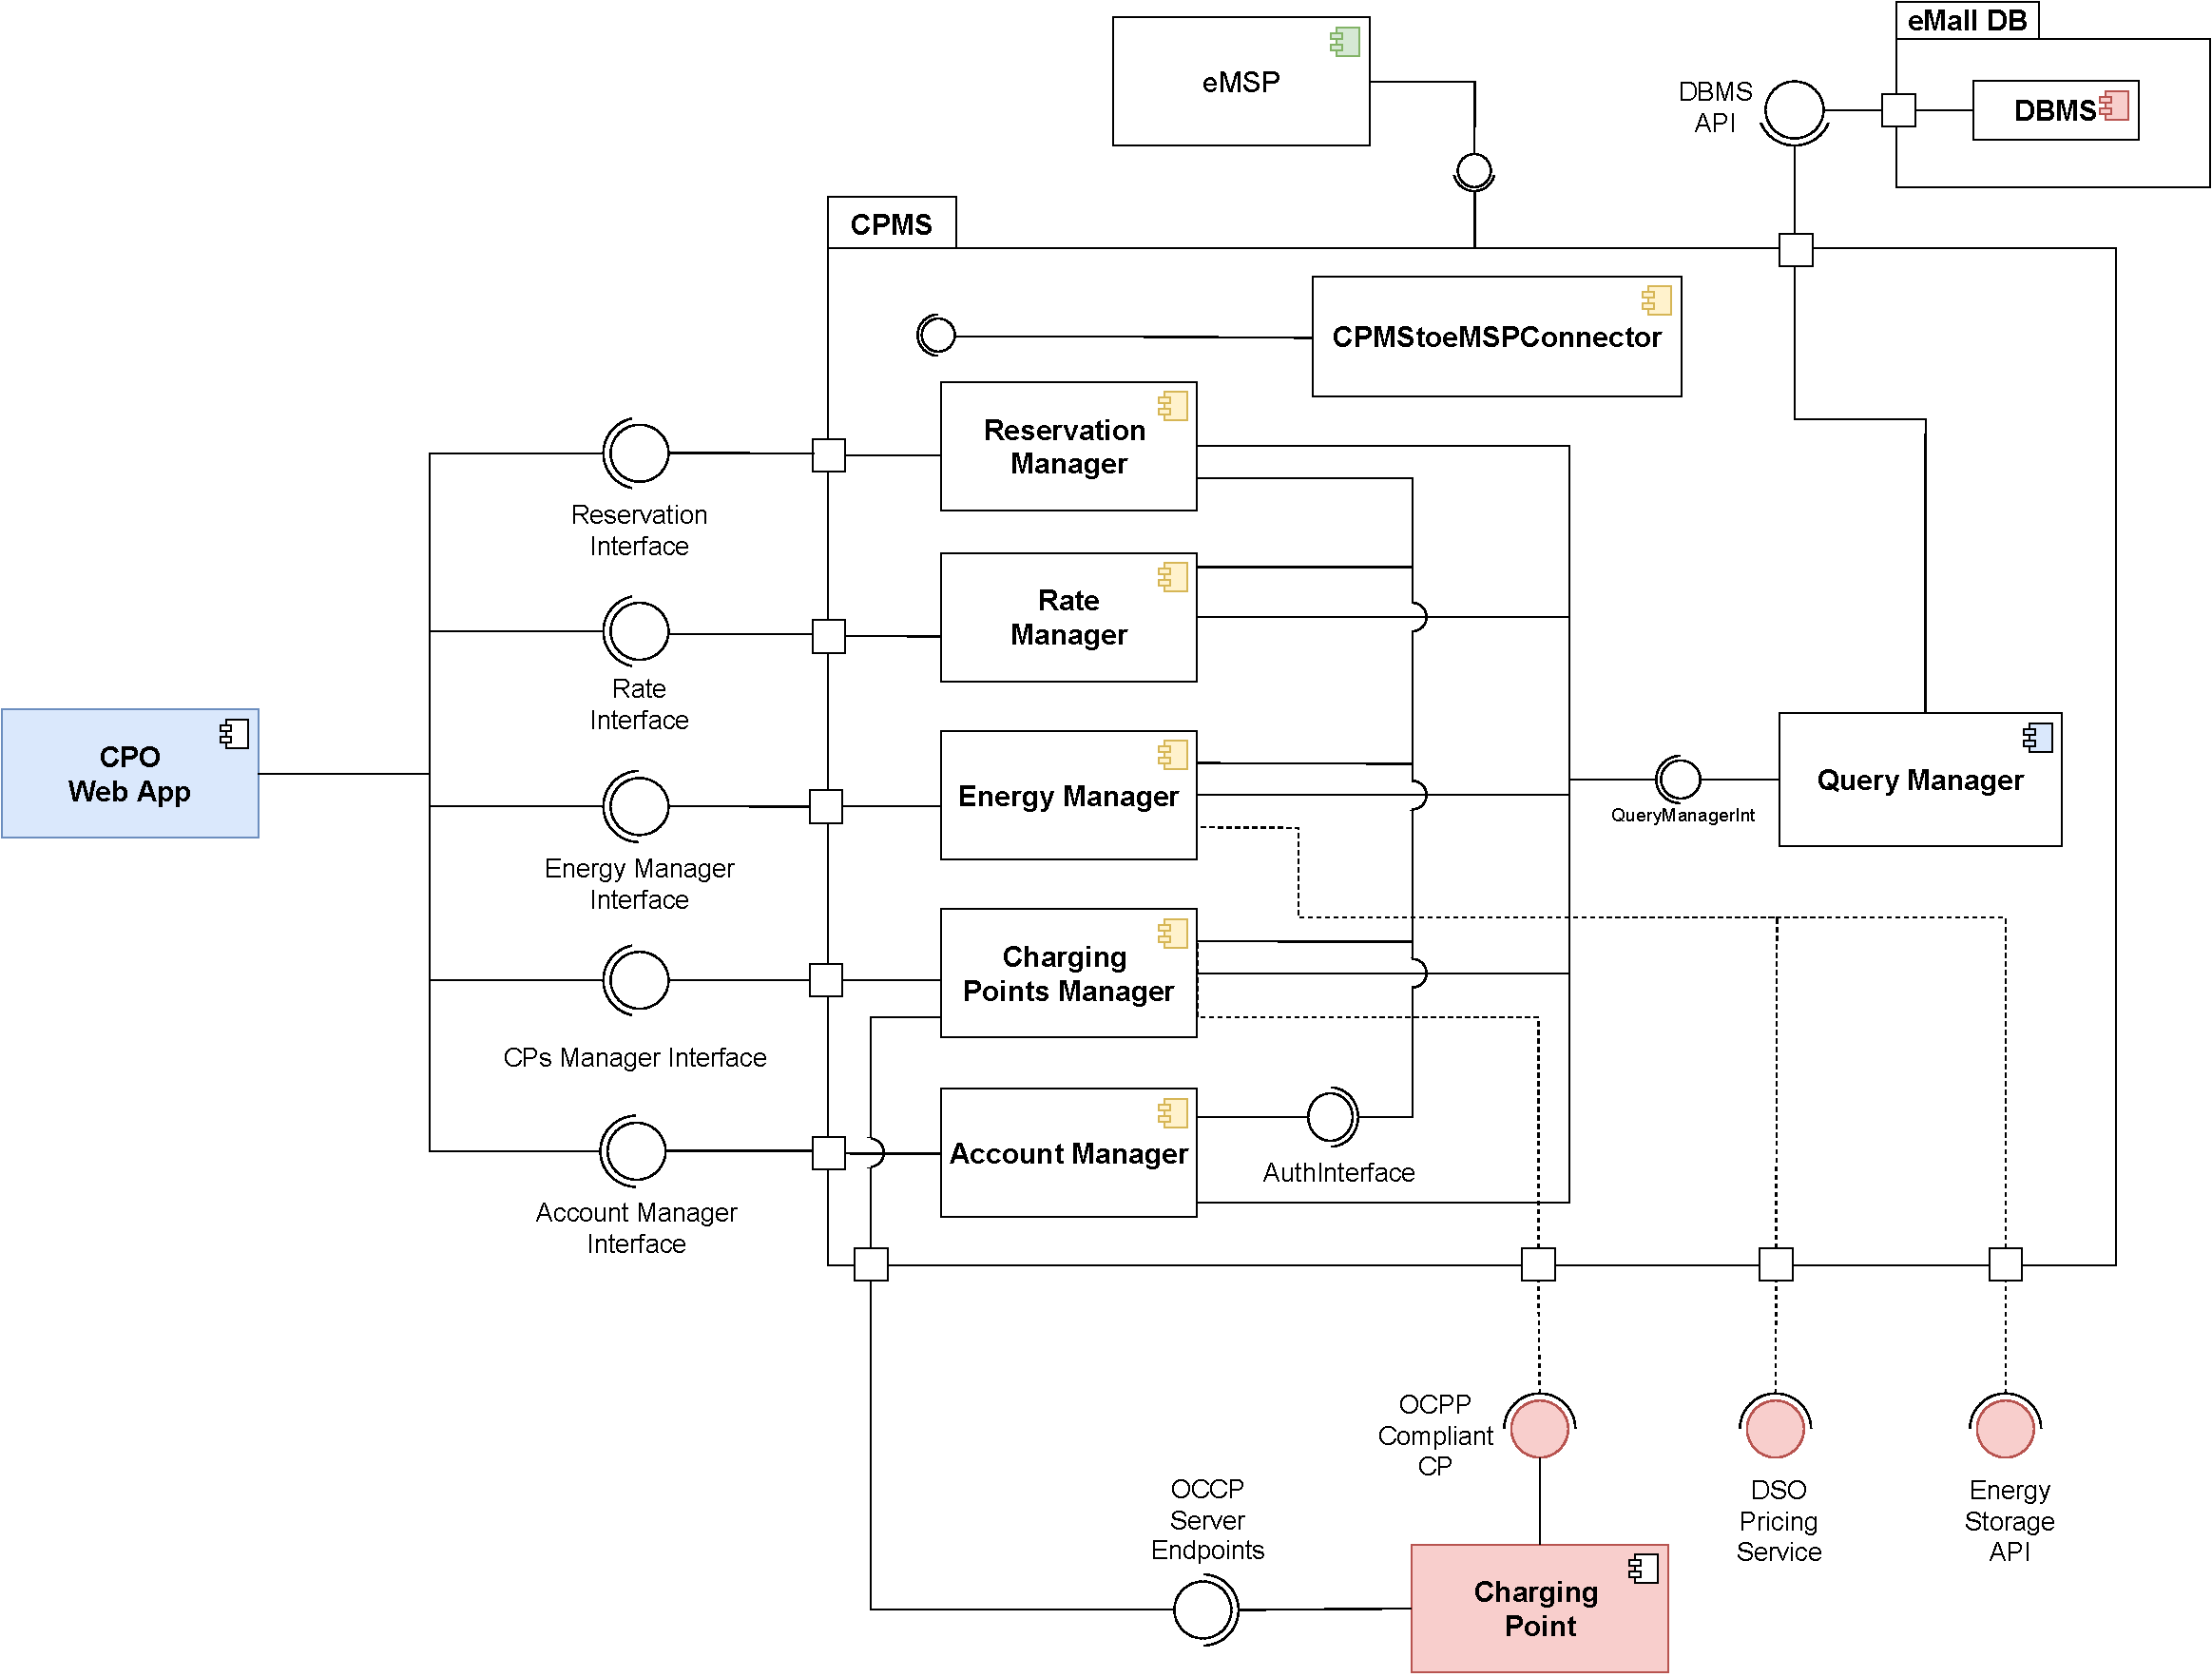
\includegraphics[scale=0.5]{src/ComponentDiagram/cpms_component_diagram.pdf}
    \caption{Component Diagram of the CPMS subsystem}
\end{figure}

\paragraph*{CPO Web App} \hfill \\
It represents the application dedicated to the different CPOs using the system. This component contains the logic to receive HTTPS requests from the users' browser,
forward them to the CPMS Application Server, and generate dynamic pages based on the response from the CPMS Application Server.

\paragraph*{CPMS Application Server} \hfill \\
The CPMS Application Server is responsible for the business logic to provide the functionality to the application for the CPOs and to coordinate the information flow between application layer and data layer.
It is composed of several components, each of them used for a specific functionality:\\
\begin{itemize}
    \item \textbf{Booking Manager} \\
          This component handles the operations regarding the reservation of a specific CPO. It offers the possibility to manage the reservations and to control their status.
    \item \textbf{Rate Manager} \\ This component is responsible for the operations regarding the rates of that are associated with the CPs. It offers the possibility to
          create a new rate in all its details, to add a special rate and specify the duration. The created rates then are associated to a specific CP.
    \item \textbf{Energy Manager} \\ This component is responsible for the operations regarding the managing of the energy of the different EVCPs.
          It offers the possibility to verify the energy consumption and production of the different sources, modify and visualize the status of the energy storage system,
          visualize the availability of energy contracts provided by the DSOs for a specific EVCP and stipulate a contract among the ones available.
    \item \textbf{Charging Points Manager} \\ This component handles the operations regarding the managing of the CPs. It is an OCPP server for the CPs, offering the
          required functionalities for adding and removing a CP, for starting and stopping a charge and for receiving status data by the CP. It offers an interface to connect the different CPs through their platform.
    \item \textbf{CPMS's Account Manager} \\ This component handles all the account operations related to the CPO and offers an interface to authenticate the requests in the CPMS application server.
          It offers functionality to create new account, logging in, setting preferences and verify the authentication of the user at any time.
          To create a new account interacts with the external SMS API to make the user receive a code to verify the identity.
\end{itemize}

\begin{figure}[H]
    \centering
    \hspace*{-2.5cm}
    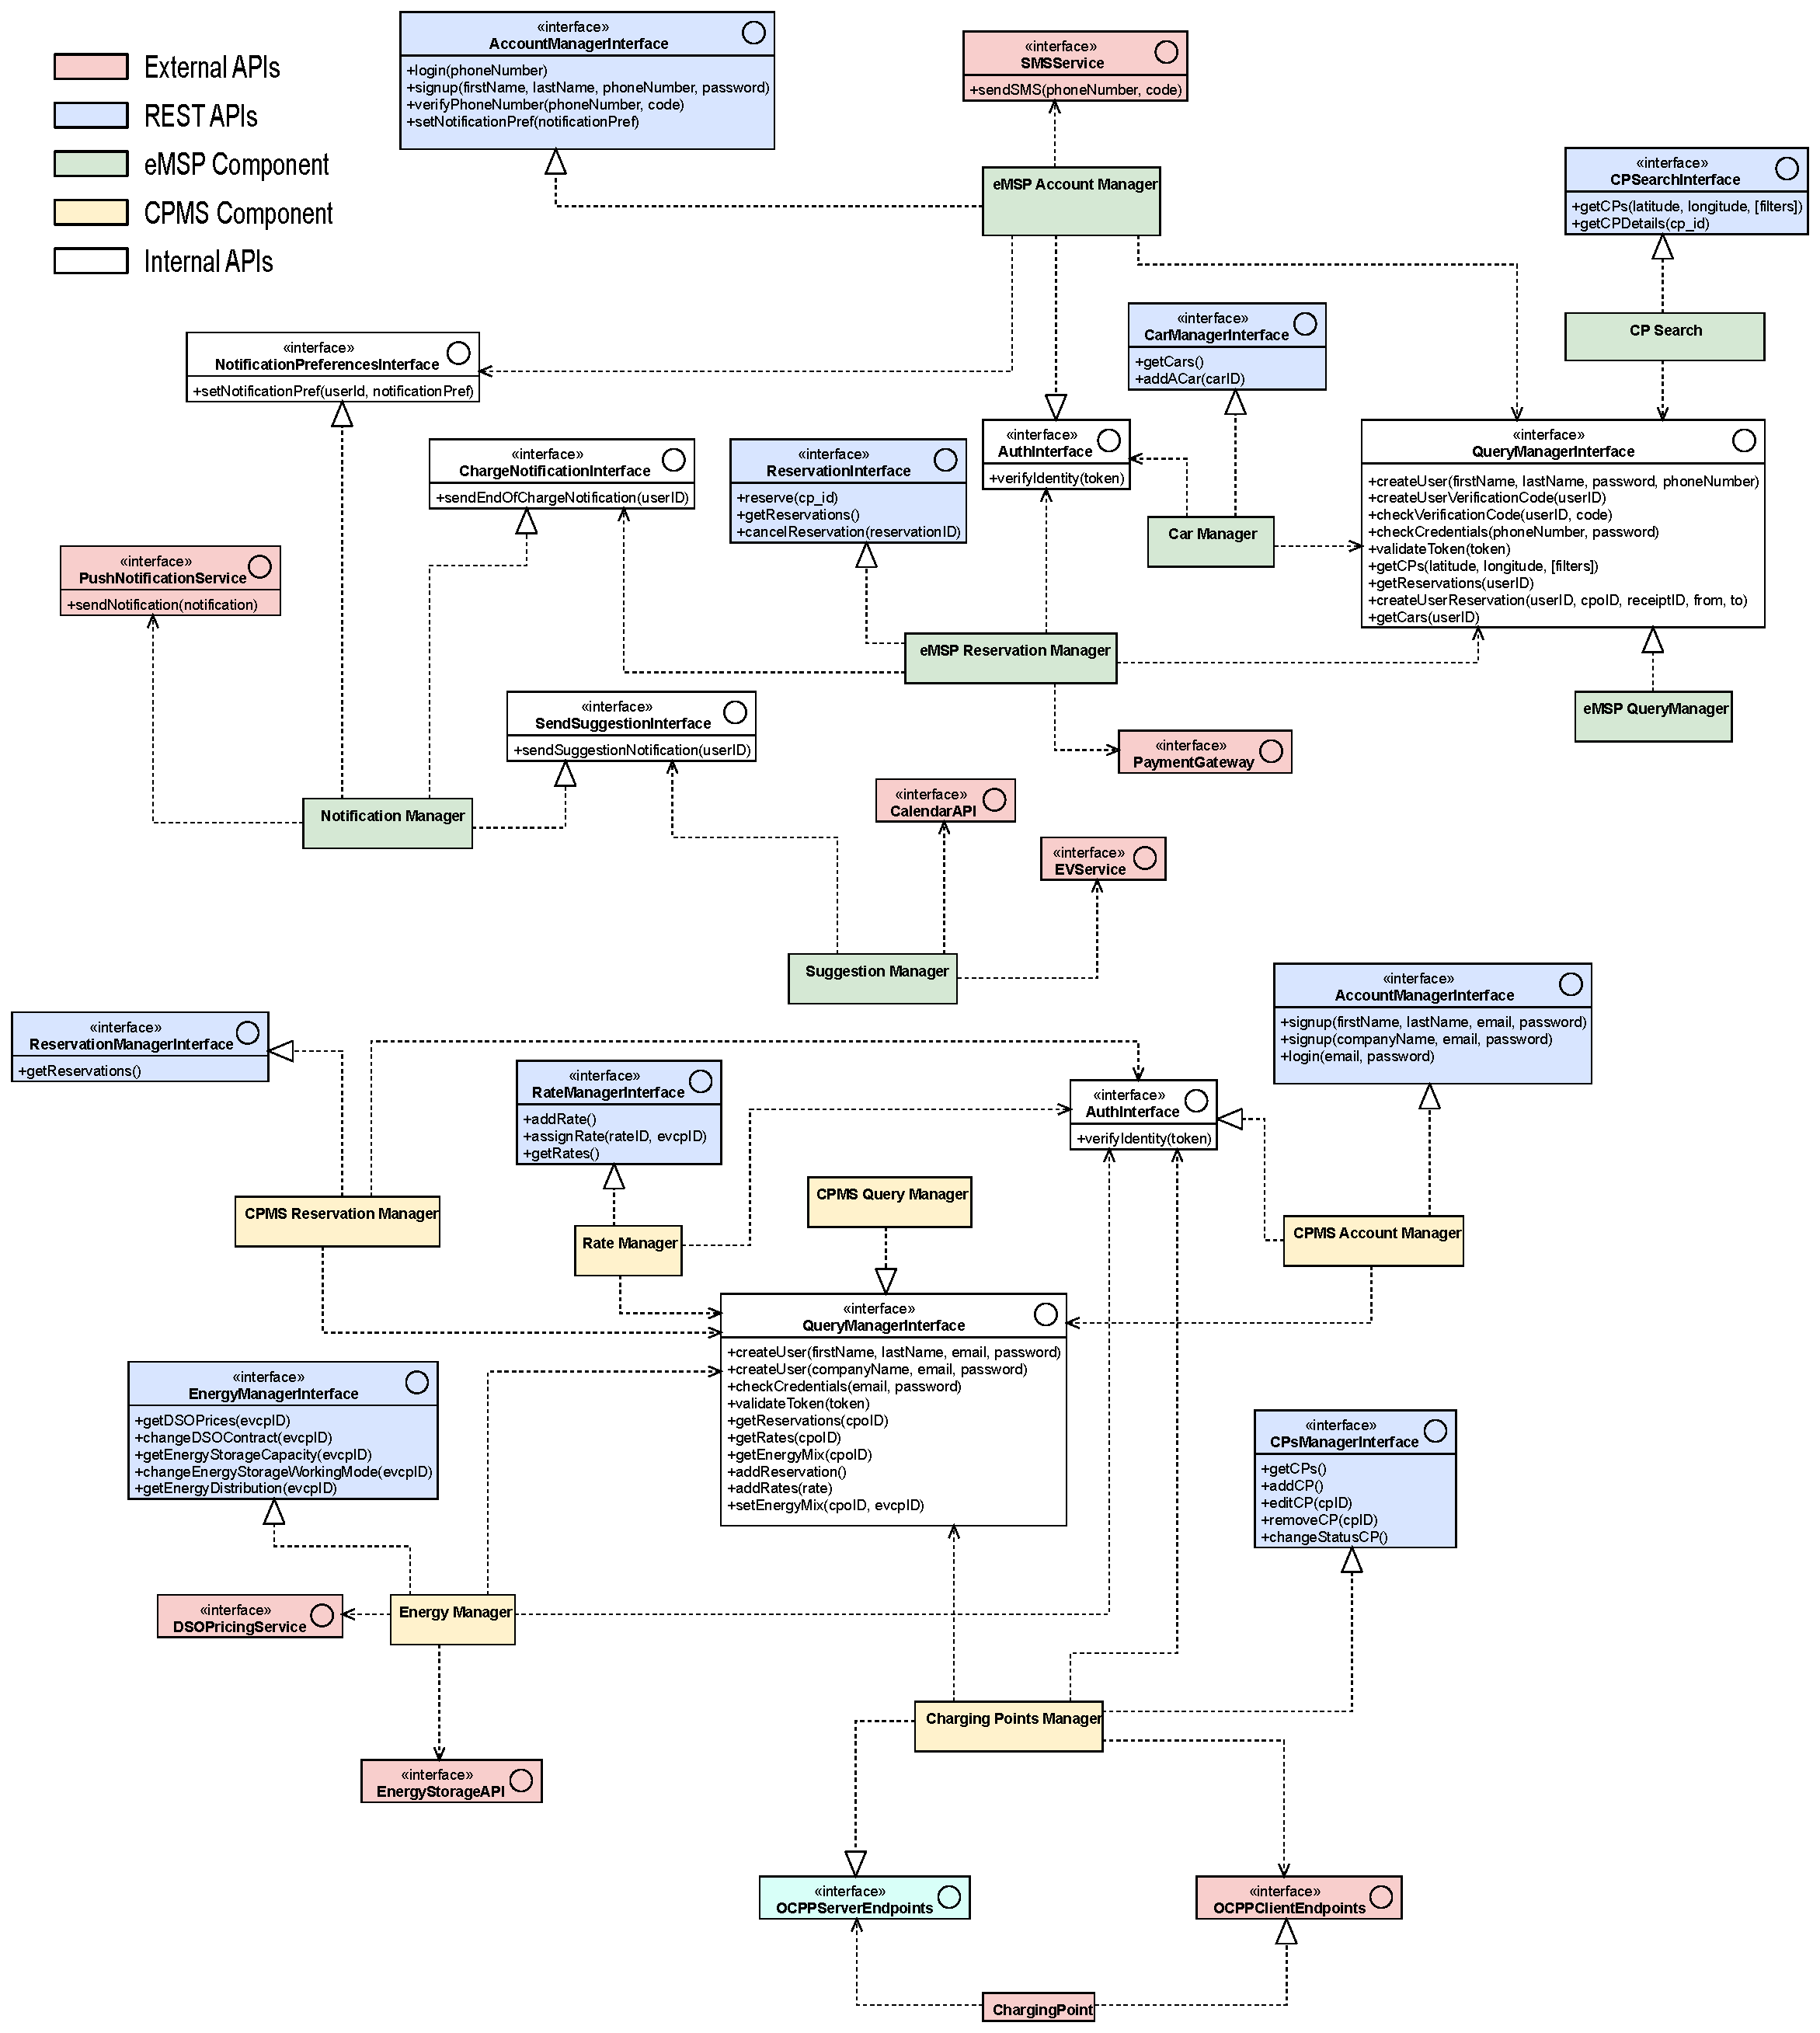
\includegraphics[height=\textheight-1.5cm,keepaspectratio]{src/componentInterfaces/component_interface.pdf}
    \caption{Class Diagram with interfaces of the eMall System}
\end{figure}


\subsubsection{Logical Description of Data}
\begin{figure}[H]
    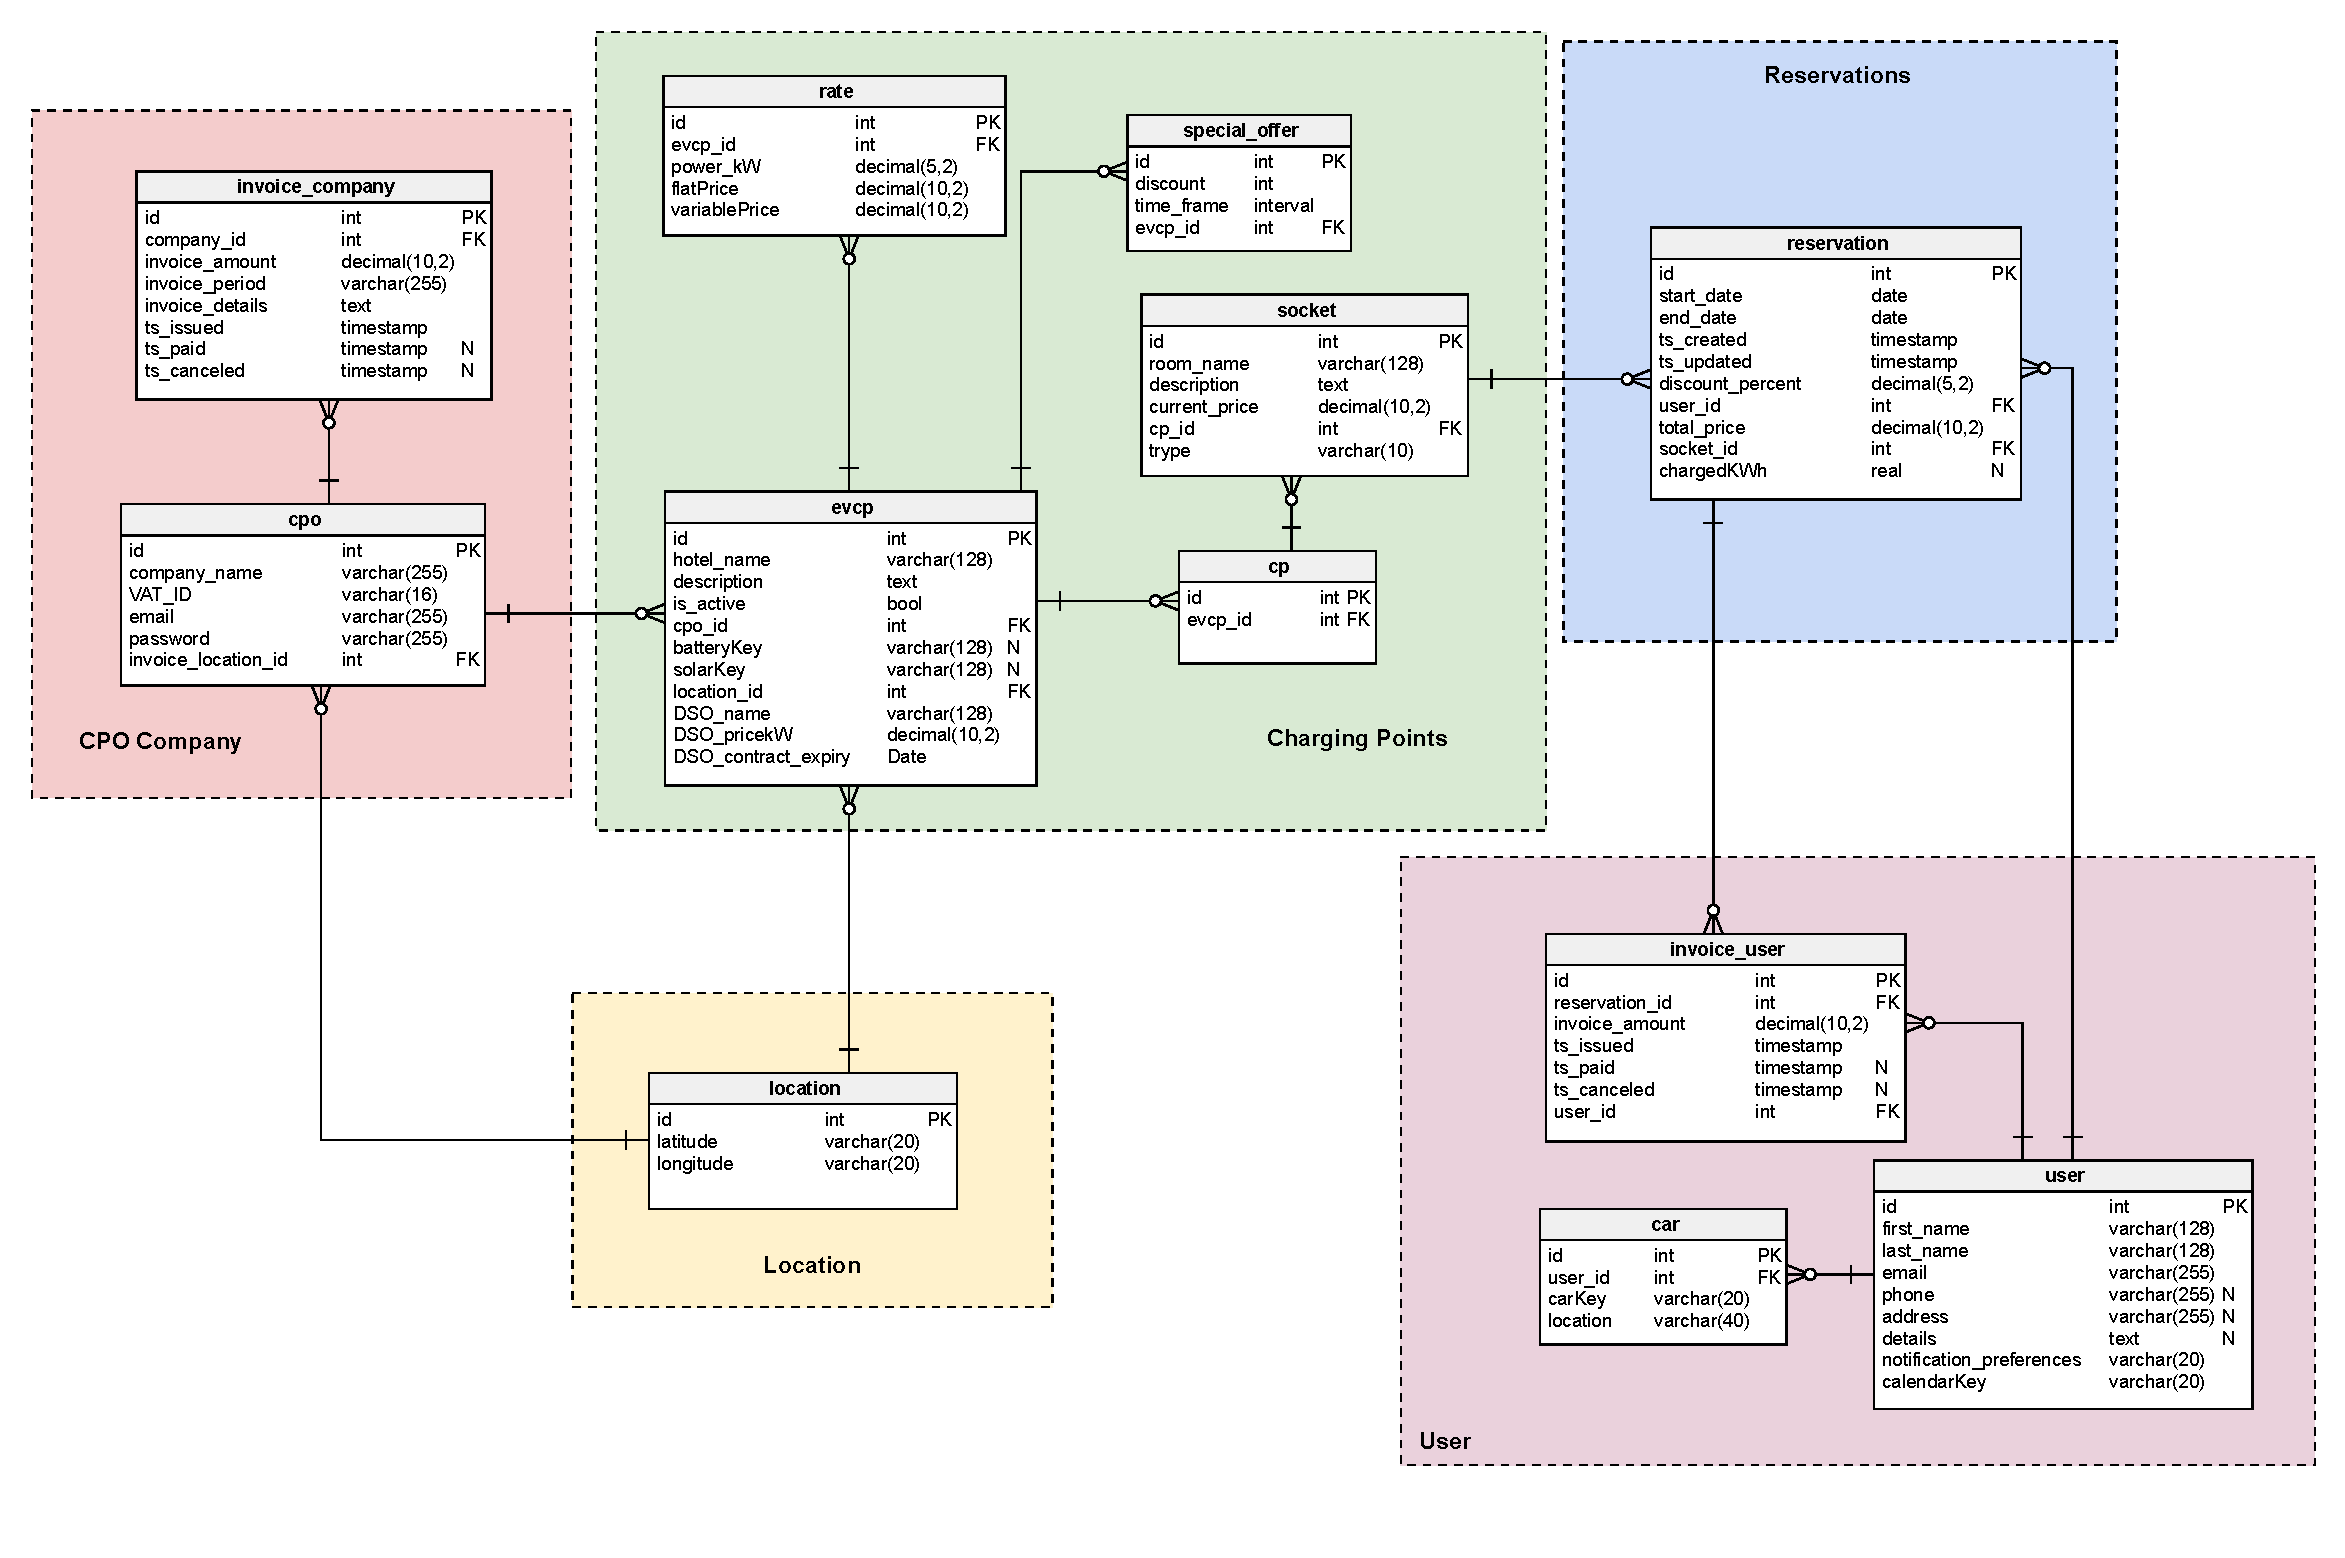
\includegraphics[scale=0.30]{src/ERDiagram/er_diagram.pdf}
\end{figure}

\subsection{Deployment view}

Our system consists of two parts: a static web server and an application server. The static web server will be the entry point for clients to access the SPA, while the application server will provide the necessary APIs for the SPA to work. We have chosen to use two different solutions for these components. The static web server will be hosted on a CDN (Content Delivery Network) to ensure fast response times through its edge location caches and reverse proxies. The application server, which includes both a business logic layer and a data tier, will be hosted on a cloud provider.
This offers several advantages compared to traditional in-house hosting, such as:
\begin{itemize}
    \item Scalability and Flexibility - the ability to add or remove resources such as virtual machines, performance cores, or memory as needed, and the use of load balancing services, allows the application server to adapt to changes in traffic or workload.
    \item Security - services like live monitoring and firewalls help to protect the application server against data breaches, cyberattacks, and other security threats.
    \item Cost-efficiency - the pay-as-you-go model of a cloud provider allows to only pay for the resources that are actually used, which can help to lower the overall costs.
\end{itemize}
These features make a cloud provider an ideal choice for hosting large, high-traffic applications. The chosen cloud provider will need to offer all of these features in order to meet our needs.

\begin{figure}[H]
    \centering
    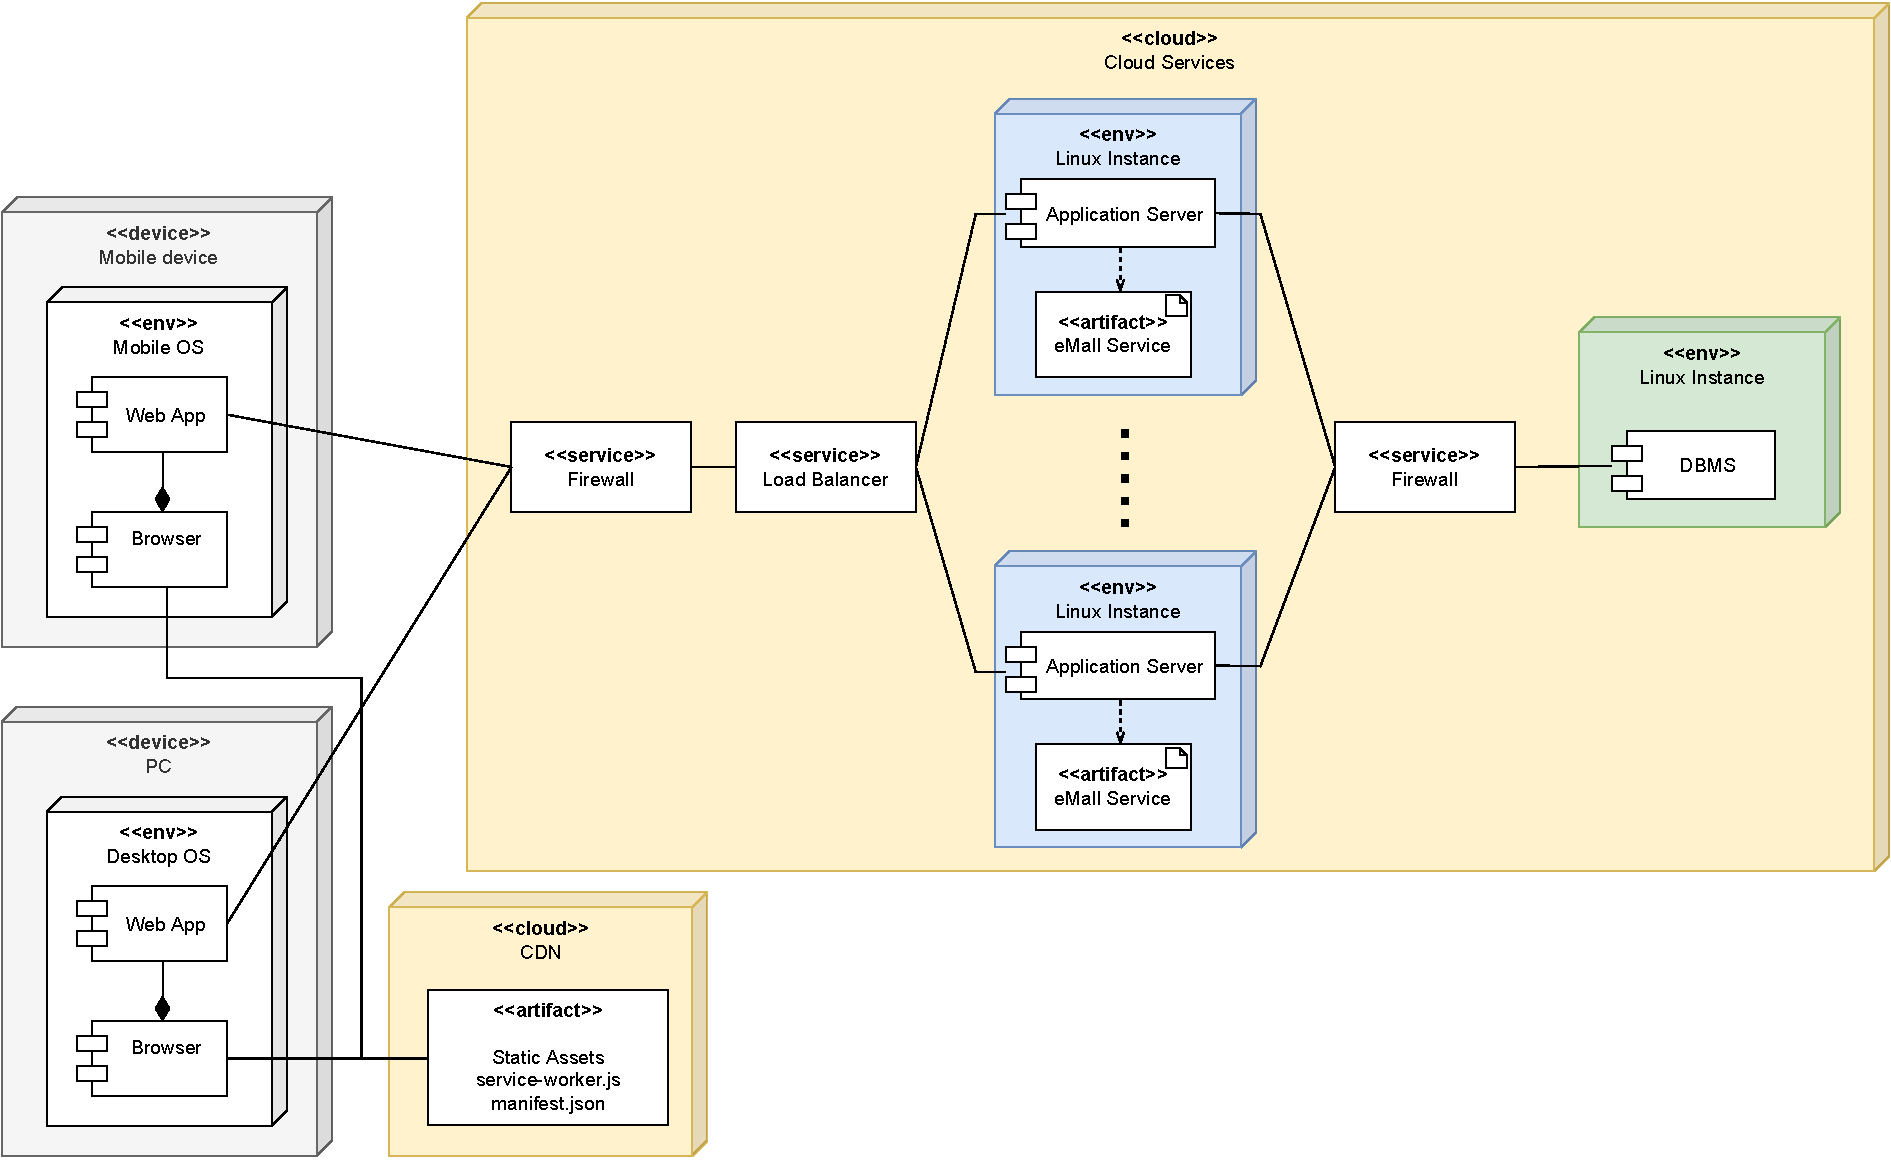
\includegraphics[scale=0.55]{src/deploymentDiagram/deployment_diagram.pdf}
    \caption{EV Driver Registration process}
\end{figure}

The deployment diagram offers a more detailed view over the hardware and software resources of the application:
\begin{itemize}
    \item PC or Mobile Device is any device having a modern browser capable of running the JavaScript based web app.
    \item The SPA will be hosted by a CDN, which will allow it to be downloaded without affecting the performance of the main application server. The SPA is static and all of its code is run on the client's machine, so there is no need for any logic to be implemented on the CDN side.
    \item The Cloud Services will host all the business and data logic for the system. It contains:
          \begin{itemize}
              \item \textbf{Firewall} services are used to filter incoming connections to the business and data layers of a system. They provide an additional layer of security by blocking or allowing traffic based on predetermined rules. This helps to protect the system from unauthorized access or malicious attacks.
              \item \textbf{Load balancer} to distribute incoming traffic across multiple instances of an application in order to optimize resource utilization, improve performance, and ensure high availability. The load balancer helps to ensure that the application can handle a large volume of requests without becoming overloaded or experiencing downtime. It also helps to provide a more stable and reliable experience for users by redirecting traffic to the least busy application instance.
              \item Multiple copies of the \textbf{application}. The various instances can run in parallel and independently to meet the demand for the application. These instances can be created or deleted as needed. Running multiple instances allows the application to handle a high volume of requests without experiencing performance issues, and provides fault tolerance by allowing traffic to be redirected to a different instance if one instance becomes unavailable.
              \item \textbf{Data Instance} which is a data optimized virtual machine containing the DBMS and the database.
          \end{itemize}
\end{itemize}



\pagebreak
\subsection{Runtime view}
The runtime view describe the interactions between actors, subsystems and interfaces of the system showing the specific method called.
The views are devided between eMSP and CPMS.

\subsubsection{eMSP}
\begin{itemize}
    \item \textbf{EV Driver Registration} : The following diagram represents the workflow that an EV Driver has to follow to register into eMall.\\
          \\When the unregistered user enters the input data the System will check wether the data input is valid. If the input is valid,
          the request is forwarded to the Account Manager that proceeds to evaluate if there is another user registered with
          the same phone number. If the user has inserted a phone number not already registered, then the user is created and an sms verification
          code is sent to the user through the SMS Service. After receiving the correct verification code the user is notified that the
          registration is completed.
          \begin{figure}[H]
              \centering
              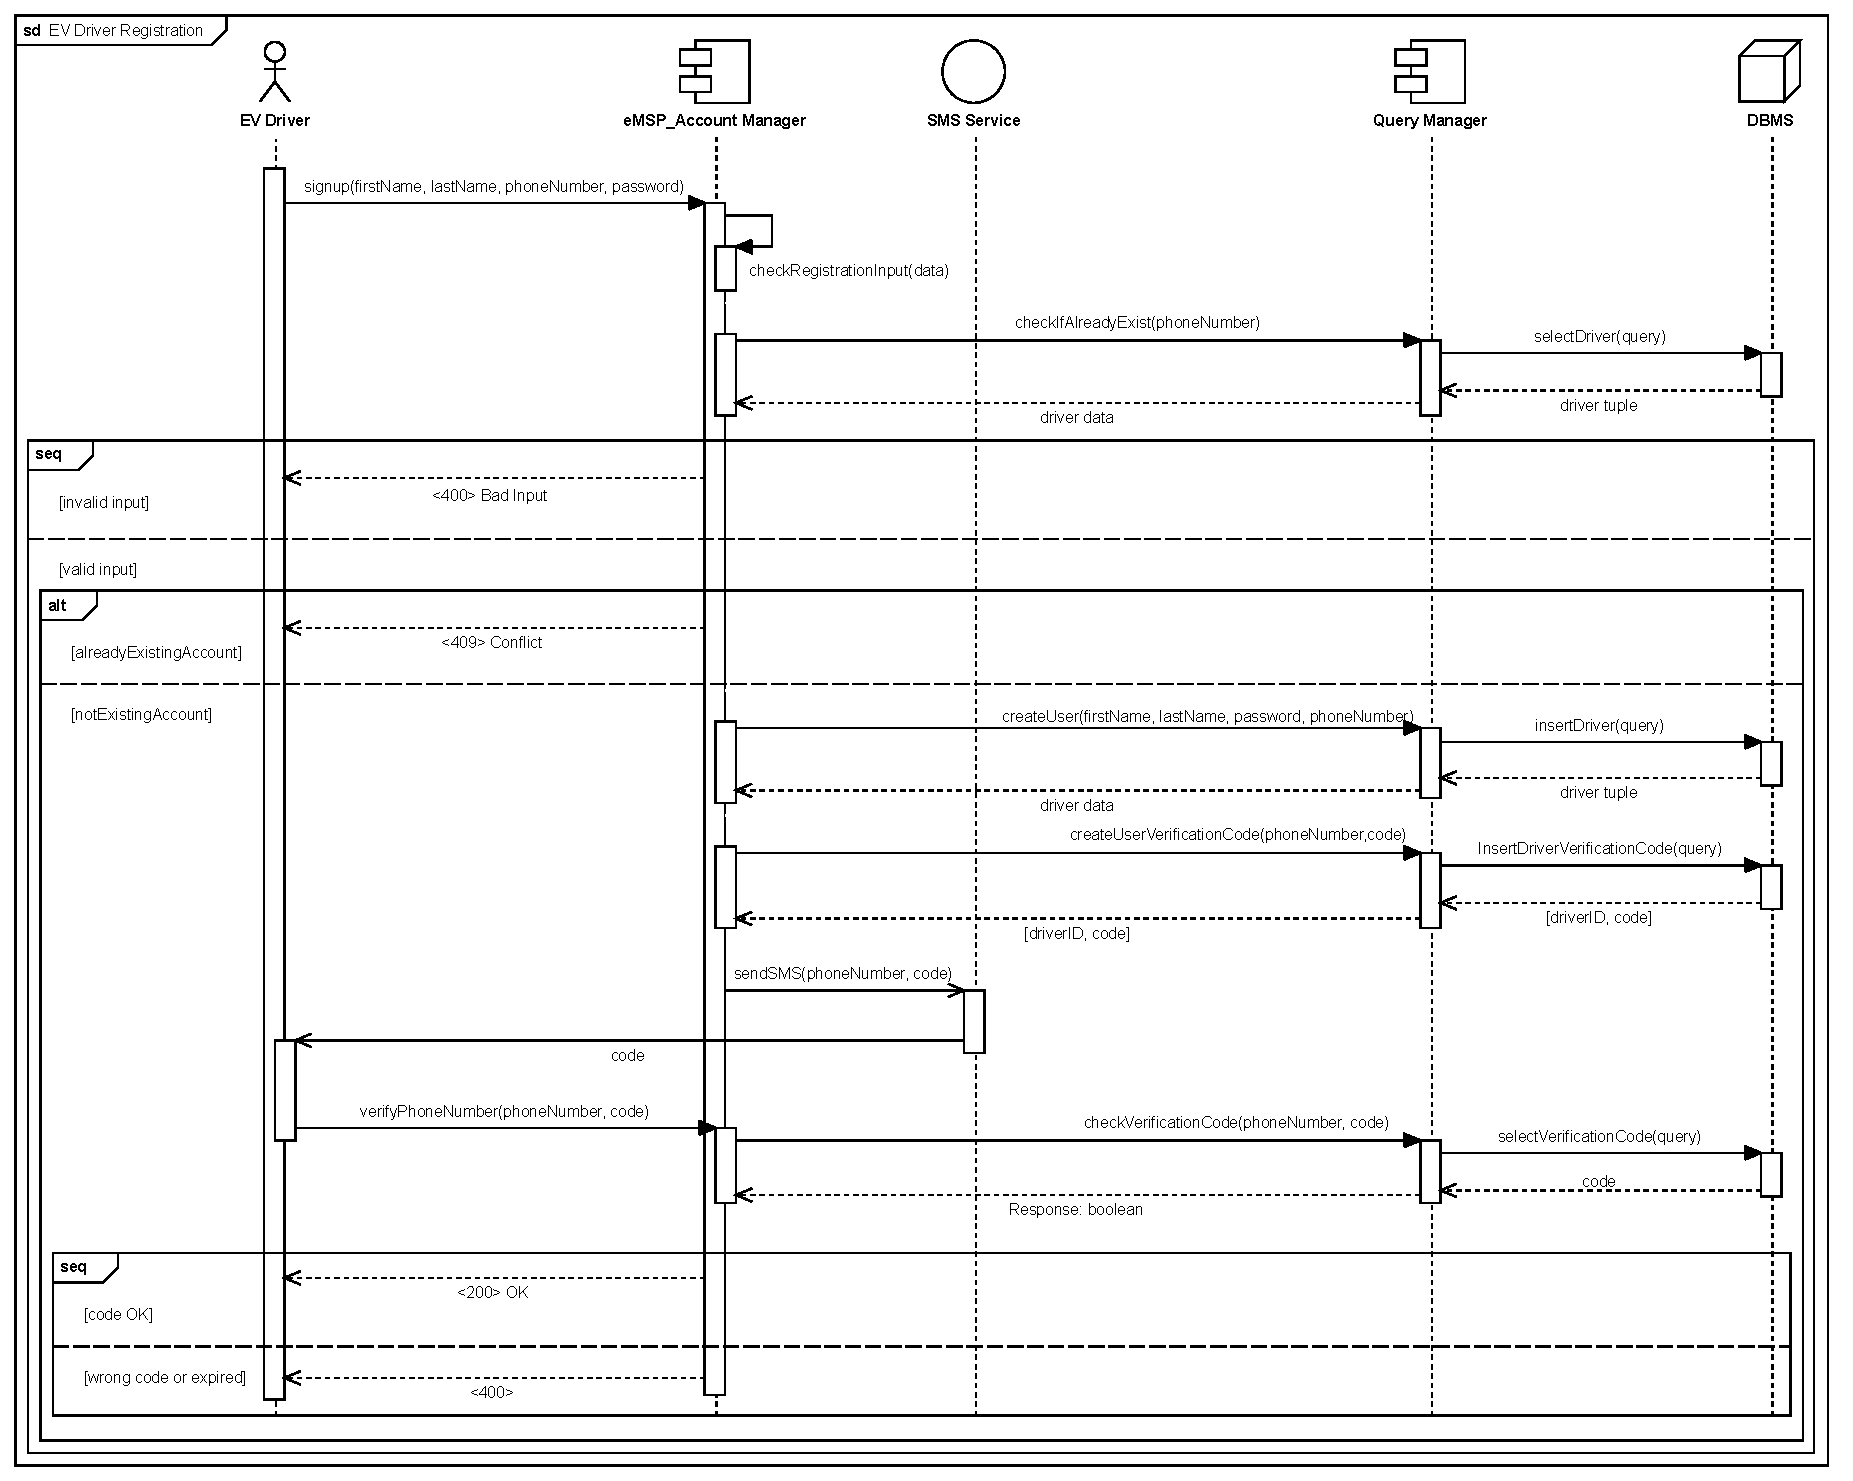
\includegraphics[scale=0.55]{src/runtimeView/eMSP_Registration.pdf}
              \caption{EV Driver Registration process}
          \end{figure}
          \pagebreak
    \item \textbf{EV Driver Log in} : The following diagram represents the workflow that the EV Driver has to follow to log in.\\
          \\After submitting the login inputs, the Account Manager verifies the credentials by interacting with the Query Manager. If
          the input is correct authenticates the user through a token and redirects the EV Driver to the Map Homepage.
          \begin{figure}[H]
              \centering
              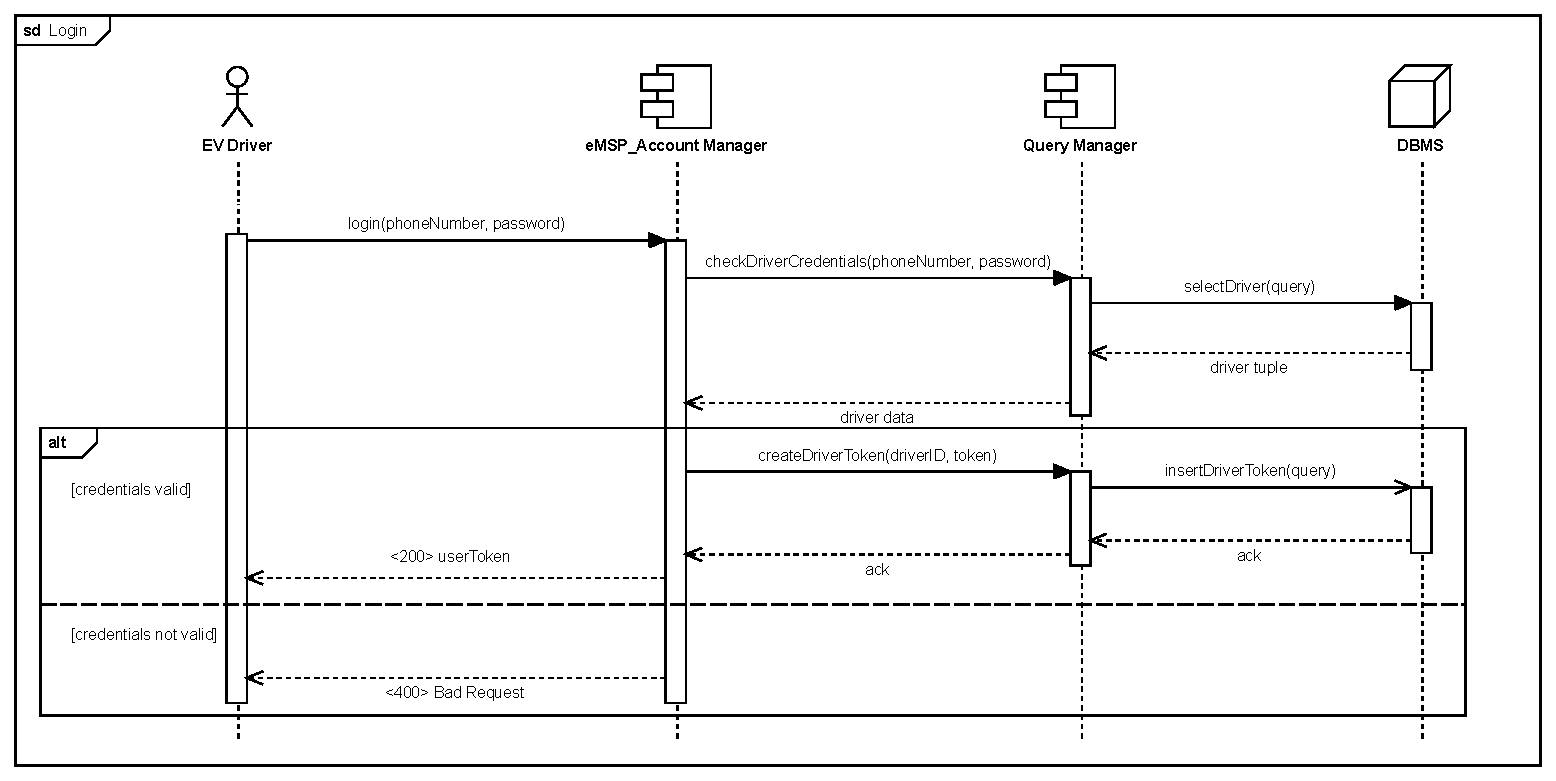
\includegraphics[scale=0.55]{src/runtimeView/eMSP_Login.pdf}
              \caption{EV Driver Logs in the system}
          \end{figure}
    \item \textbf{EV Driver Search} : The following diagram represents the workflow that the EV Driver has to follow to search for CPs in the map.\\
          \\By filtering the results by location, connector and/or date sends a request for an update of the page. The CP Search
          interacts with the Query Manager to get the filtered CPs and responds with the list.

          \begin{figure}[H]
              \centering
              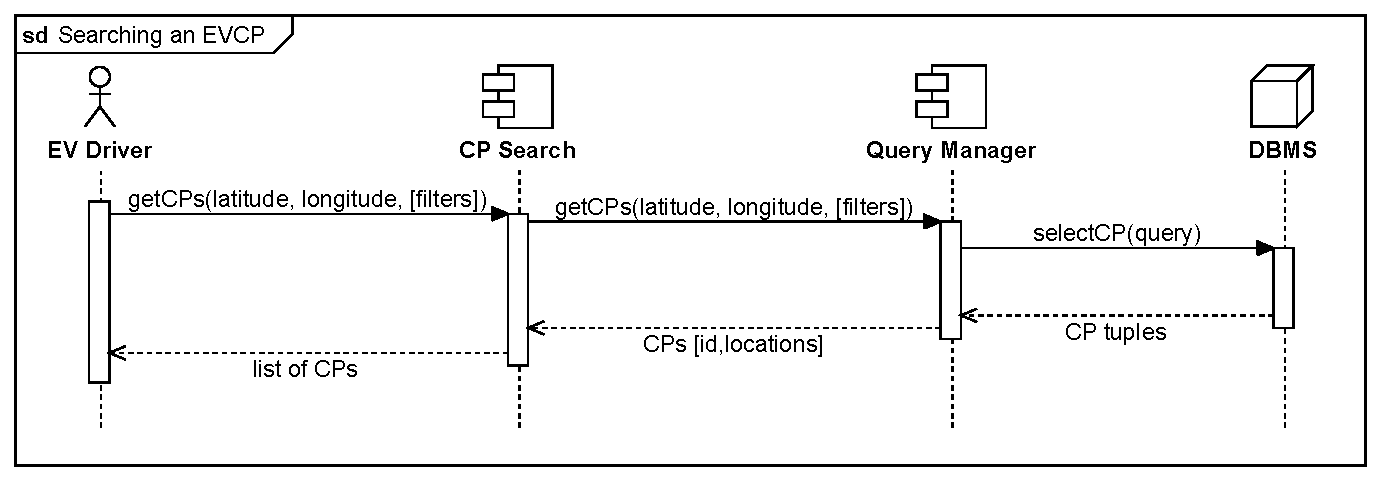
\includegraphics[scale=0.55]{src/runtimeView/eMSP_Search.pdf}
              \caption{EV Driver searches on the map}
          \end{figure}
          \pagebreak
    \item \textbf{EV Driver books a charge} : The following diagram represents the workflow when the EV Driver books a charge.\\
          \\After the submission of the reservation parameters by the user, the Reservation Manager interacts with the eMSPtoCPMSConnector to
          contact the specific CPMS to book the charge. The reservations parameters are received by the specific CPMStoeMSPConnector that
          forwards the payload to the Booking Manager that contacts the Query Manager to verify that the reservations parameters aren't in
          conflict with others reservations. If the reservation is valid then is added to the database through the Query Manager and the Reservation
          Manager of the eMSP is notified of the validity of the reservation. The Reservation Manager contacts the Payment Gateway to pre authorize the
          payment with the credit card that has been already added and selected by the EV Driver.
          \begin{figure}[H]
              \centering
              \hspace*{-2cm}
              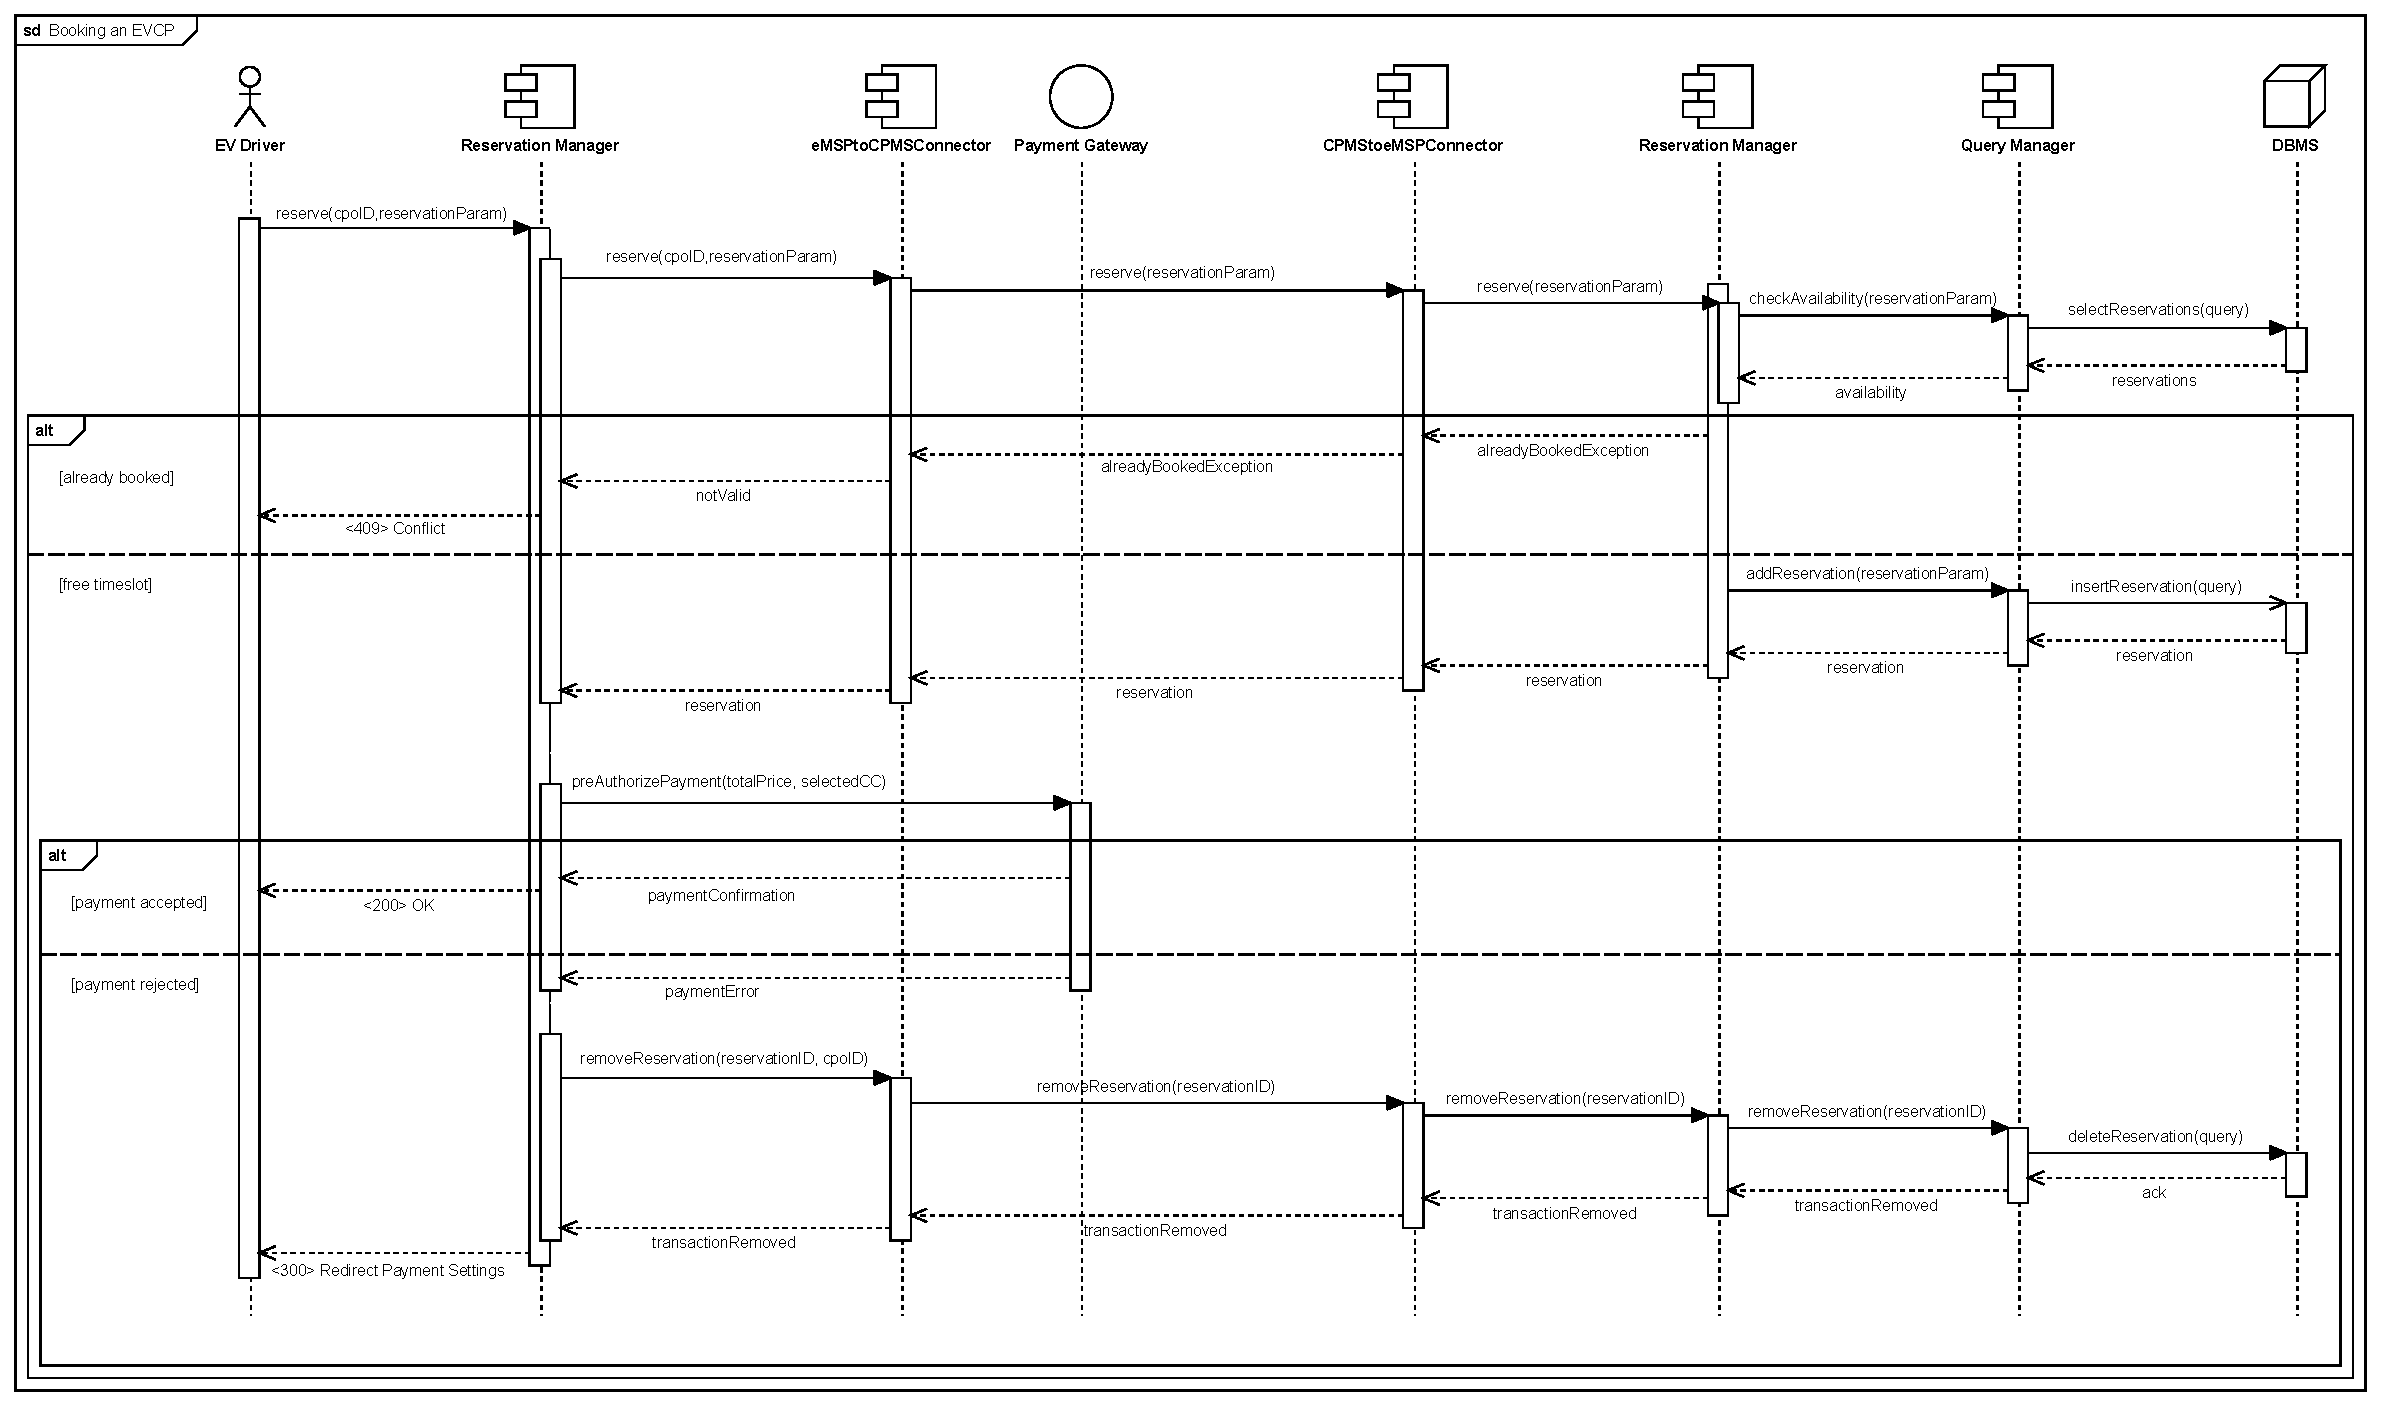
\includegraphics[scale=0.48]{src/runtimeView/eMSP_Book.pdf}
              \caption{EV Driver books a charge}
          \end{figure}
          \pagebreak
    \item \textbf{EV Driver starts a charge} : The following diagram represents the workflow when the EV Driver starts a charge.\\
          \\The submission of the request contains the reservation identifier of the charge that has to be started and the car details.
          The Reservation manager interacts with the eMSPtoCPMSConnector to contact the specific CPMS. Through the CPMStoeMSPConnector the
          Booking Manager receives the request to start a charge. Verifies through the Query Manager that the request corresponds to a reservation
          that can be started. If so, the Booking Manager contacts the Charging Points Manager to activate the socket of the CP specified in the reservation.
          The Charging Points Manager contacts the CP through the OCPP Compliant CP interface and starts the charge.
          \begin{figure}[H]
              \centering
              \hspace*{-2cm}
              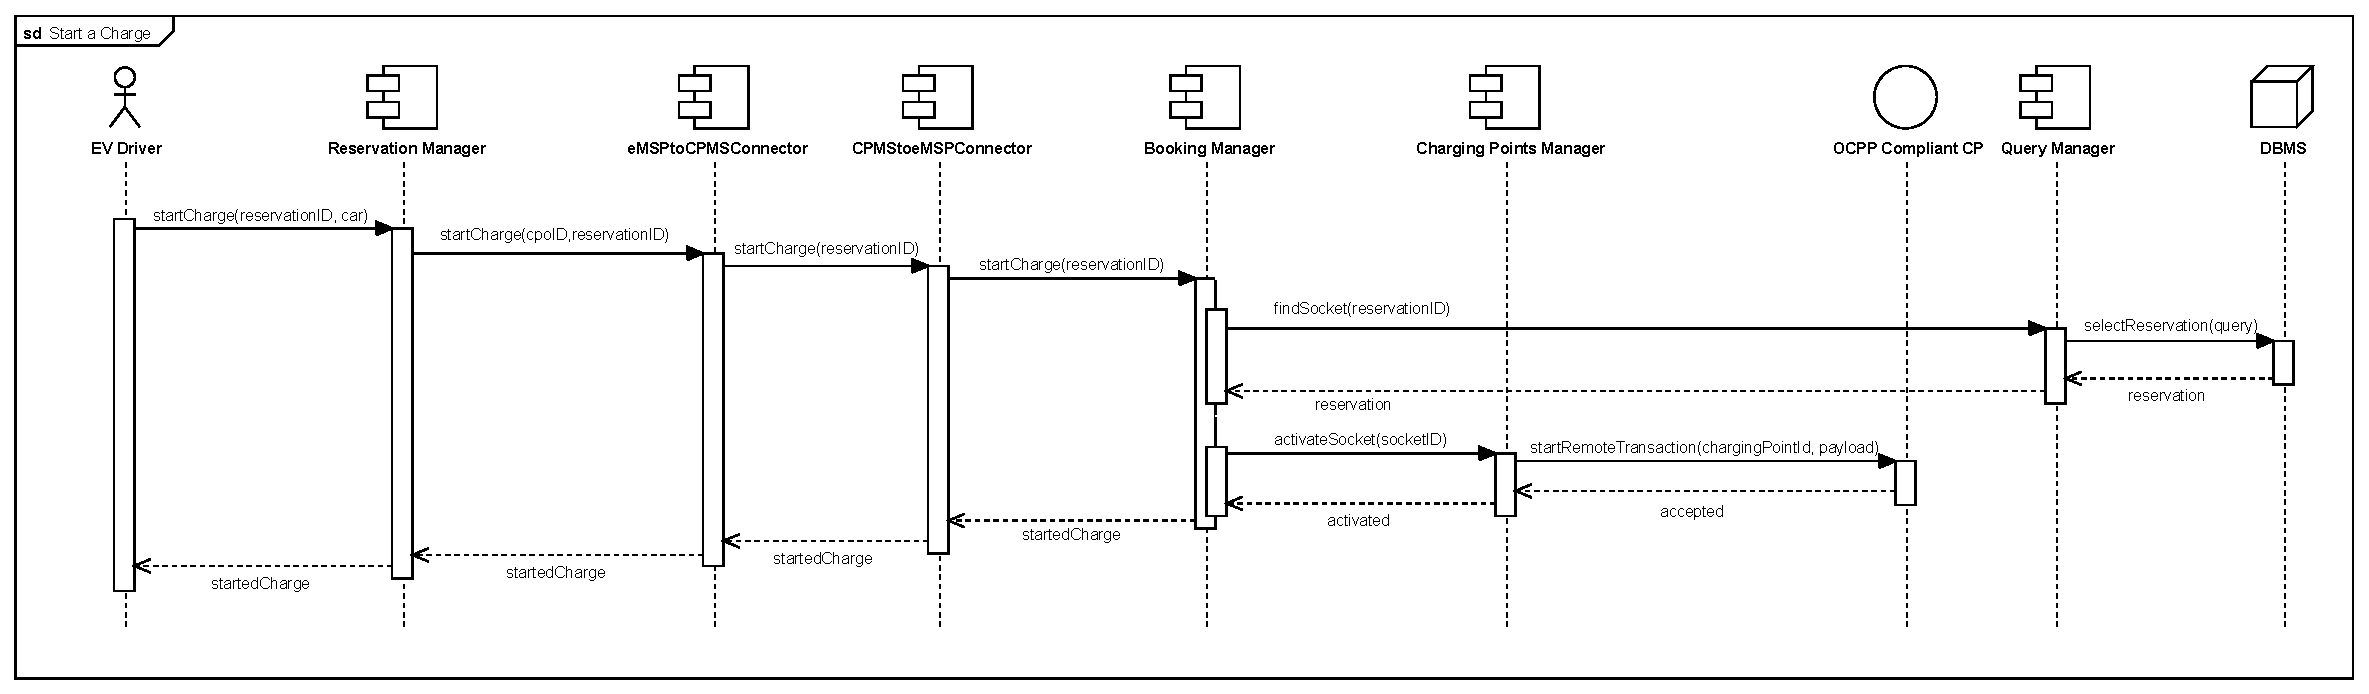
\includegraphics[scale=0.50]{src/runtimeView/eMSP_StartACharge.pdf}
              \caption{EV Driver starts a charge}
          \end{figure}
    \item \textbf{EV Driver sees reservations} : The following diagram represents the workflow when the EV Driver wants to see the his/her reservations.\\
          \\ The Reservation Manager is contacted and requires the Query Manager to find all the reservations associated with the EV Driver.
          \begin{figure}[H]
              \centering
              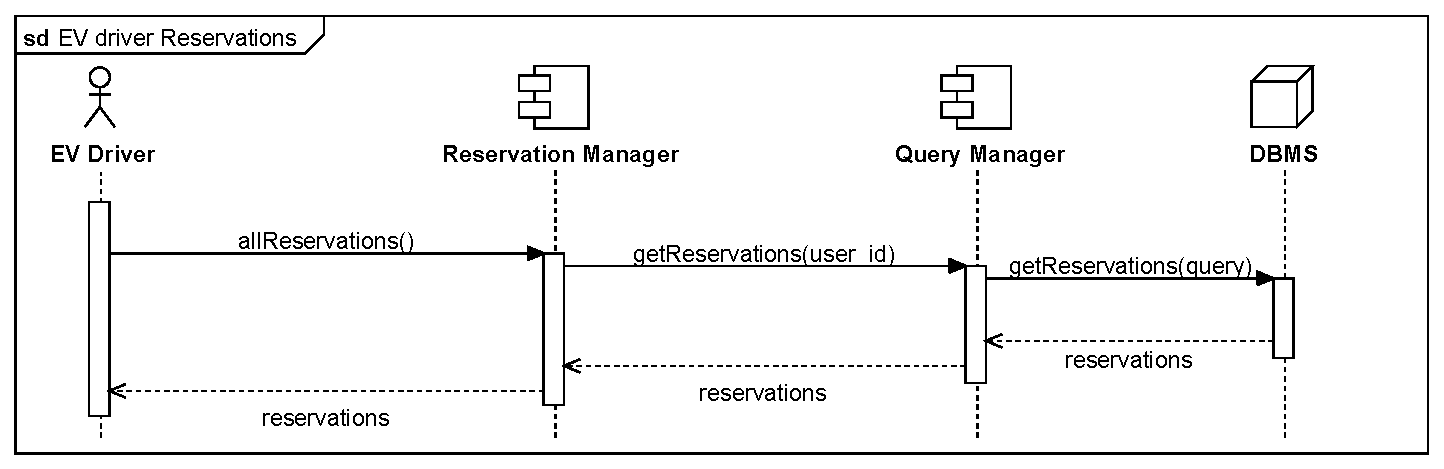
\includegraphics[scale=0.55]{src/runtimeView/eMSP_Reservations.pdf}
              \caption{EV Driver sees the reservations}
          \end{figure}
          \pagebreak
    \item \textbf{EV Driver adds a credit card} : The following diagram represents the workflow when the EV Driver adds a credit card.\\
          \\
          \begin{figure}[H]
              \centering
              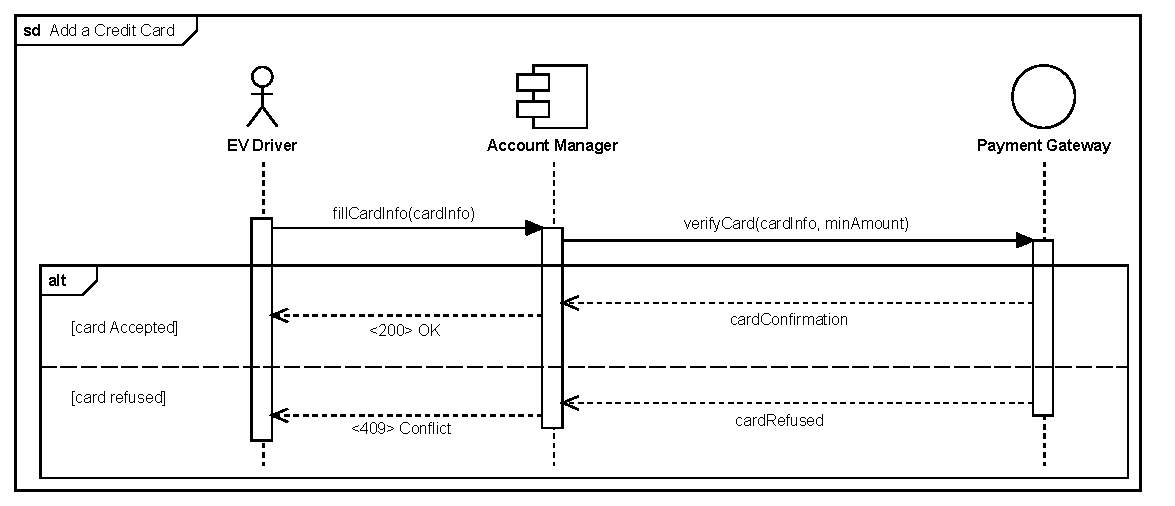
\includegraphics[scale=0.55]{src/runtimeView/eMSP_AddCC.pdf}
              \caption{EV Driver adds a credit card information}
          \end{figure}

    \item \textbf{Suggestion} : The following diagram represents the workflow when a Suggestion is sent to the EV Driver.\\
          \\After the discharge of the car, the interface EVService sends "lowBatteryEvent".
          The Suggestion Manager receives carID such that can obtain through the Query Manager, from the DB, the corresponding userID.
          The Suggestion Manager, thanks to the attribute calendar "key" of the user, interacts with the Calendar API and receives "FreeSpots" (those
          time intervals in the user Calendar that are free).
          The Suggestion Manager contacts the Query Manager with "getTopKSuggestions" through which obtains the top K suggestions according
          to the ranking implemented from the system.
          The Suggestion Manager contacts Notification Manager through which contacts the Query Manager to find the notification preferences.
          If the notification preferences of the user are such that he accepts suggestion, the Notification Manager pushes a notification through the Push Notification Service.
          \\
          \begin{figure}[H]
              \centering
              \hspace*{-2cm}
              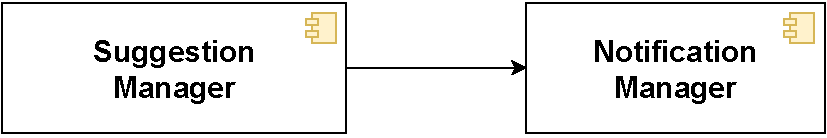
\includegraphics[scale=0.48]{src/runtimeView/eMSP_Suggestion.pdf}
              \caption{Suggestion}
          \end{figure}

    \item \textbf{Current Charge Info}: description
          \\\begin{figure}[H]
              \centering
              \hspace*{-2cm}
              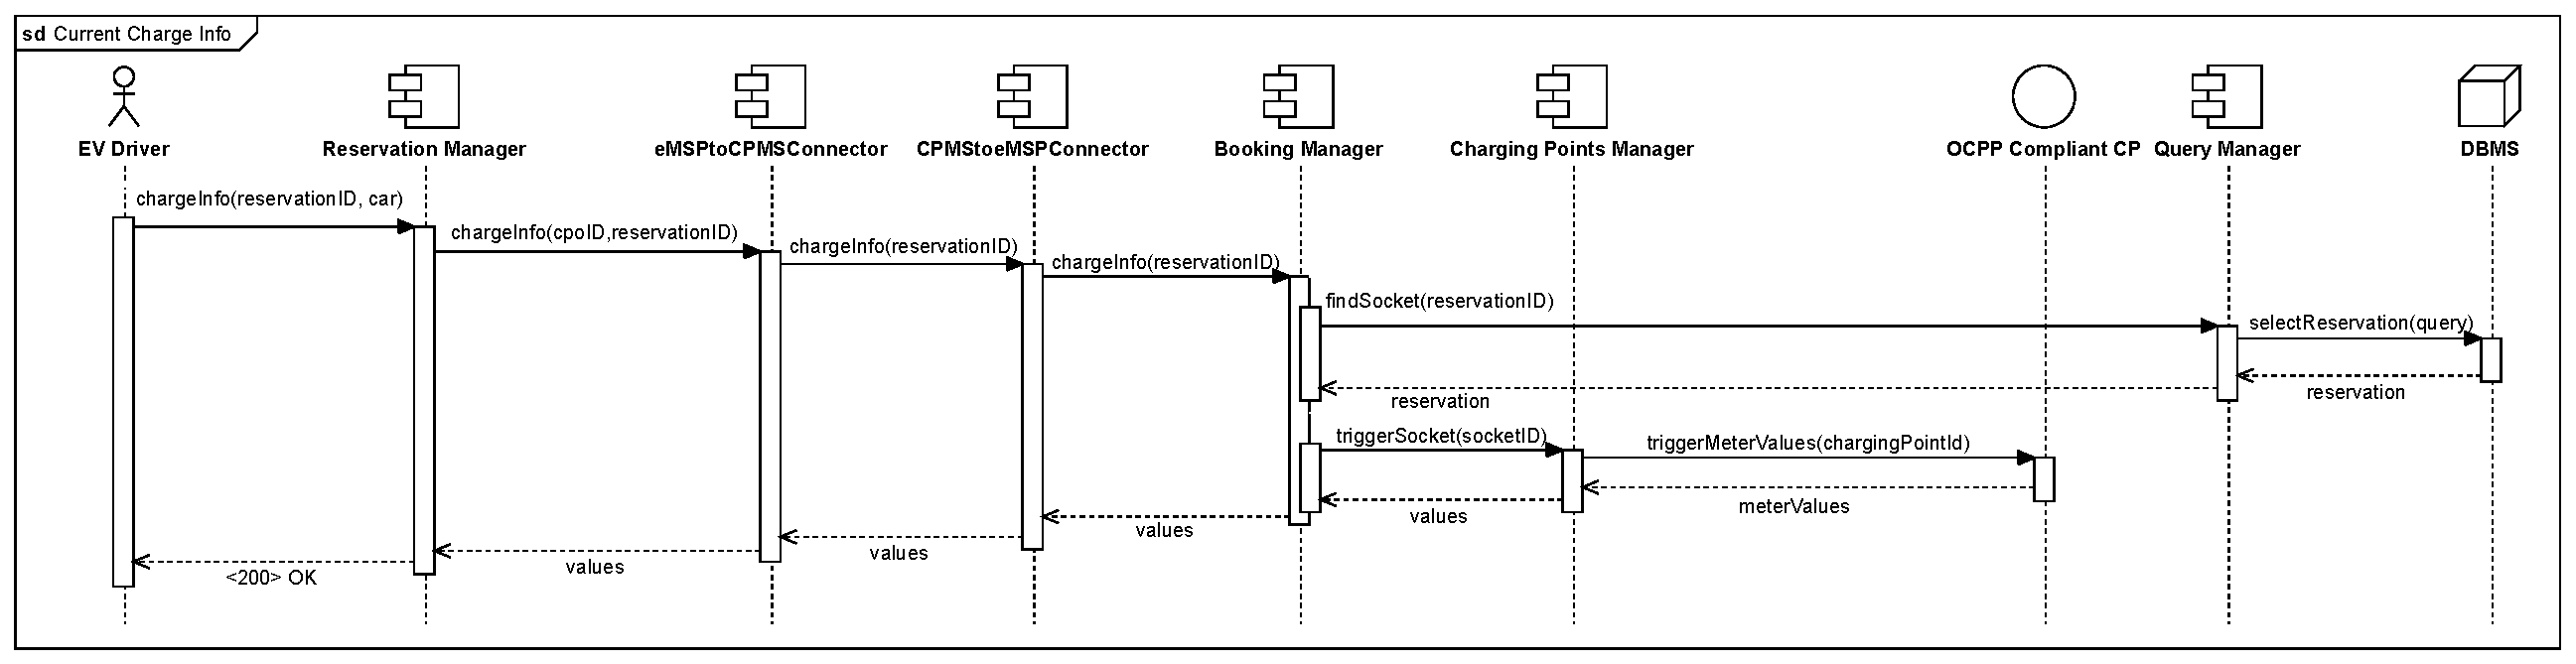
\includegraphics[scale=0.44]{src/runtimeView/eMSP_currentChargeInfo.pdf}
              \caption{EV Driver books a charge}
          \end{figure}
\end{itemize}

\subsubsection{CPMS}
\begin{itemize}
    \item \textbf{CPO sees the reservations} : The following diagram represents the workflow when the CPO wants to see the his/her reservations.\\
          \begin{figure}[H]
              \centering
              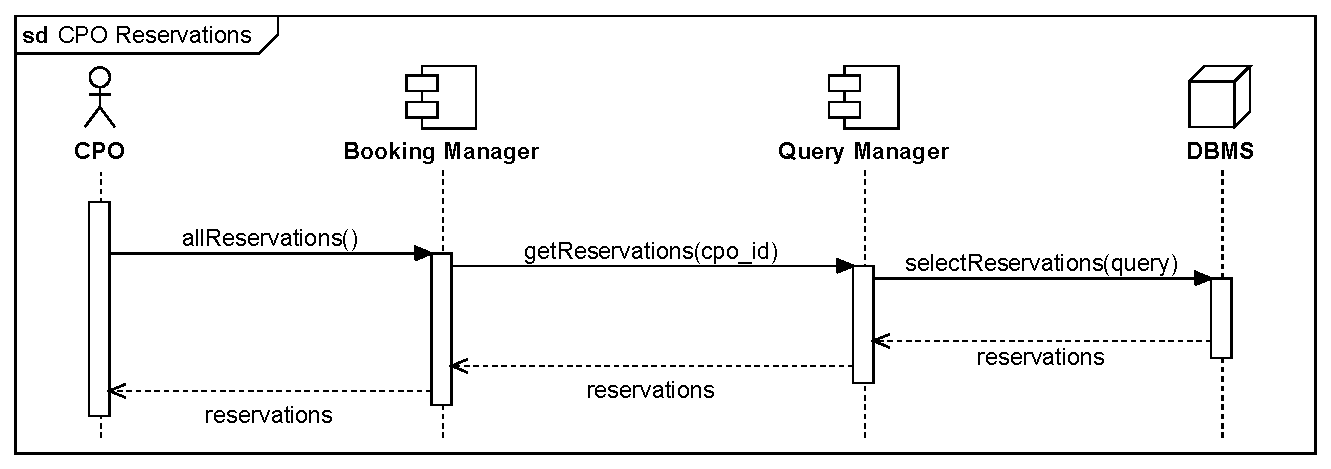
\includegraphics[scale=0.55]{src/runtimeView/CPMS_Reservations.pdf}
              \caption{CPO sees the reservations}
          \end{figure}
          \pagebreak
    \item \textbf{CPO adds a Charging Point} : The following diagram represents the workflow when the CPO adds a charging point.\\
          \\ The request contains the information about the CP unique identifier, the EVCP in which the CP is going to be added and the rate associated with.
          The Charging Points Manager interacts with the Query Manager to add the information. When the user, through the CP manufacturer's portal connects the
          CP to the CPMS, then the CP is connected and is able to receive OCPP messages from the CPMS of the CPO.
          \begin{figure}[H]
              \centering
              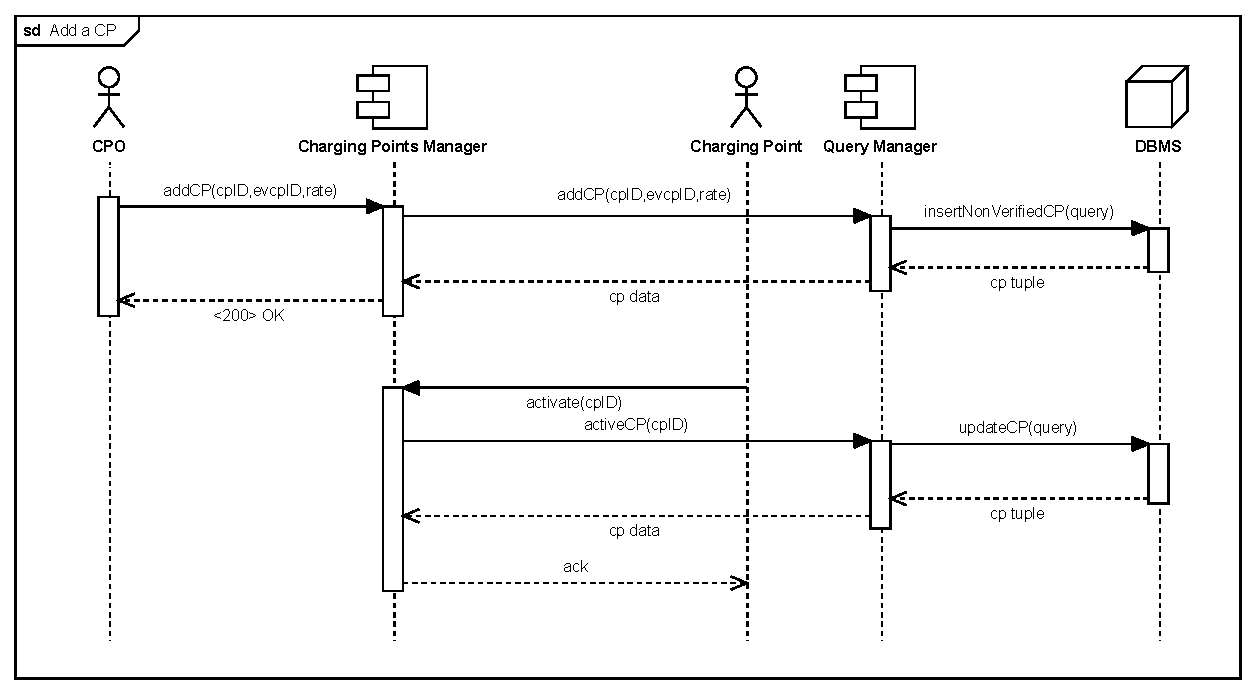
\includegraphics[scale=0.55]{src/runtimeView/CPMS_AddCP.pdf}
              \caption{CPO adds a Charging Point}
          \end{figure}
    \item \textbf{CPO adds a rate} : The following diagram represents the workflow when the CPO adds a rate.\\
          \\
          \begin{figure}[H]
              \centering
              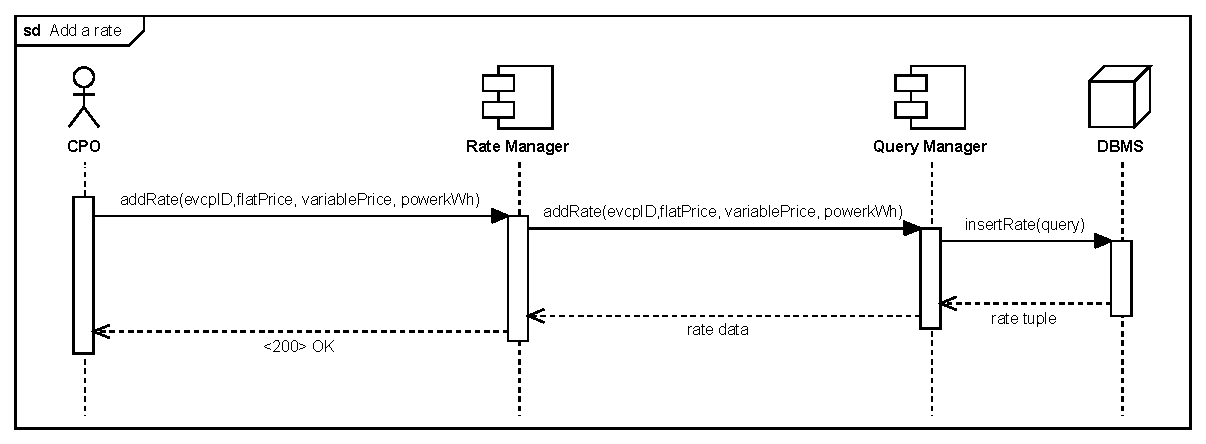
\includegraphics[scale=0.55]{src/runtimeView/CPMS_addRate.pdf}
              \caption{CPO adds a rate}
          \end{figure}
          \pagebreak
    \item \textbf{CPO sees the energy storage system capacity} : The following diagram represents the workflow when the CPO wants to see the energy storage system capacity.\\
          \\ The request contains the specific EVCP identifier of where the energy storage system is located. The Energy Manager requires to the database the unique key to access
          to the API of the Energy Storage. Then asks the Energy Storage API the information about the status.
          \begin{figure}[H]
              \centering
              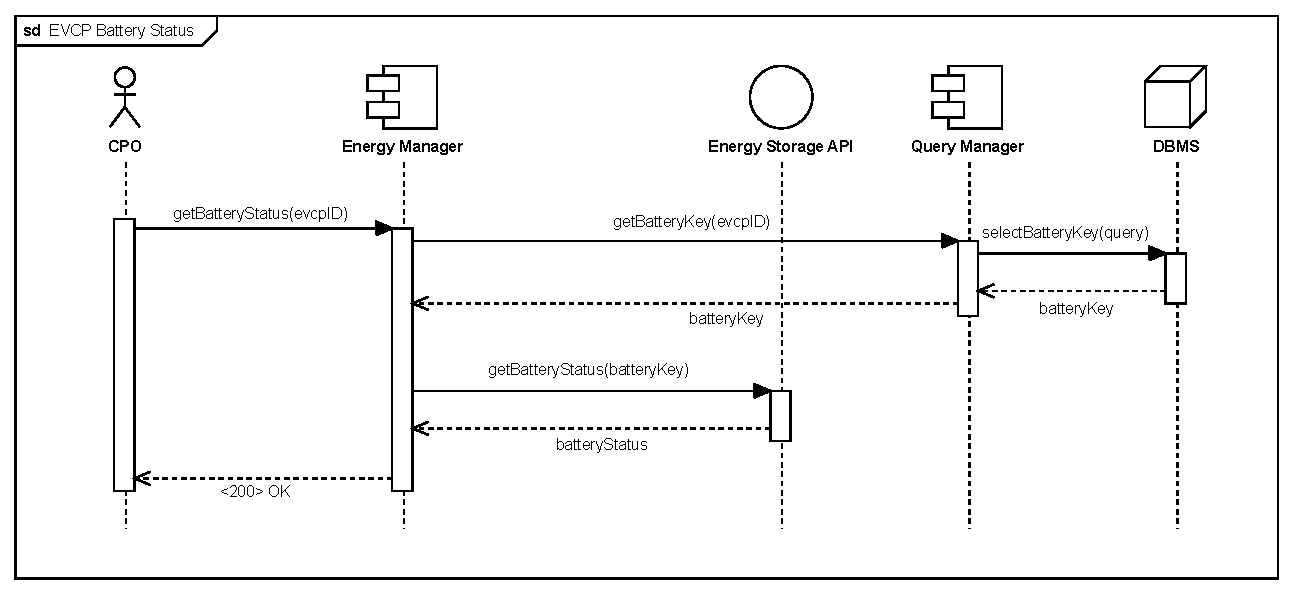
\includegraphics[scale=0.55]{src/runtimeView/CPMS_batteryCapacity.pdf}
              \caption{CPO sees the energy storage system capacity}
          \end{figure}
    \item \textbf{CPO sees the status of its Charging Points} : The following diagram represents the workflow when the CPO wants to see the charging points status of an evcp.\\
          \\ The request contains the specific EVCP identifier of where the CPs are located. The Charging Points manager asks the Query Manager for a list of CPs of the specific EVCP
          and the contacts each one of the CP from the list with the OCPP Compliant CP interface.
          \pagebreak
          \begin{figure}[H]
              \centering
              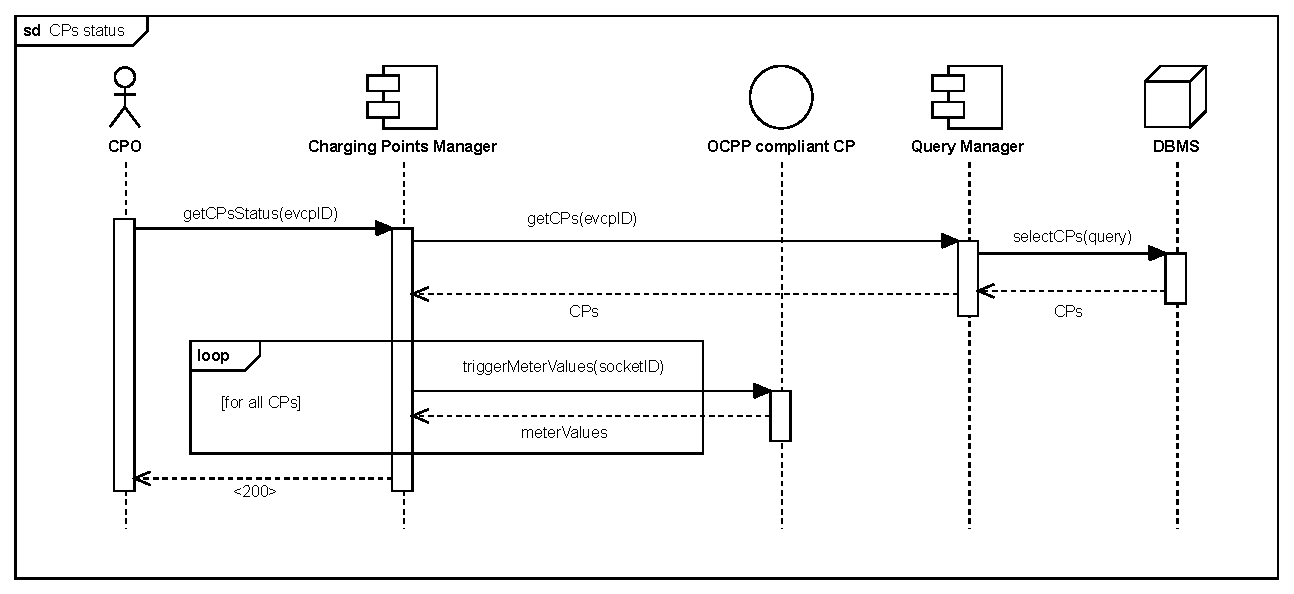
\includegraphics[scale=0.55]{src/runtimeView/CPMS_CPsStatus.pdf}
              \caption{CPO sees the status of its Charging Points}
          \end{figure}
    \item \textbf{CPO adds a special offer} : The following diagram represents the workflow when the CPO adds a special offer.\\
          \\
          \begin{figure}[H]
              \centering
              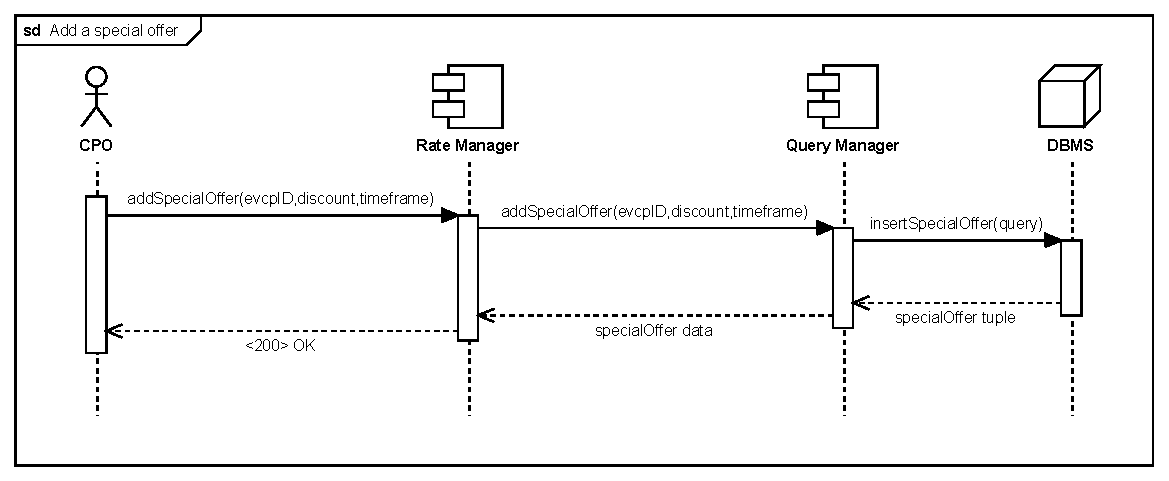
\includegraphics[scale=0.55]{src/runtimeView/CPMS_specialOffer.pdf}
              \caption{CPO adds a special offer}
          \end{figure}
    \item \textbf{Choose energy Mix} : The following diagram represents the workflow when the CPO chooses the energy mix.\\
          \\ The CPO changes energy mix interacting with the Energy Manager. The Energy Manager interacts with the Query Manager obtaining the battery and solar keys.
          Then, the Energy Manager with these informations and the mix attribute contacts the Energy Storage API and obtains the new mix.
          \begin{figure}[H]
              \centering
              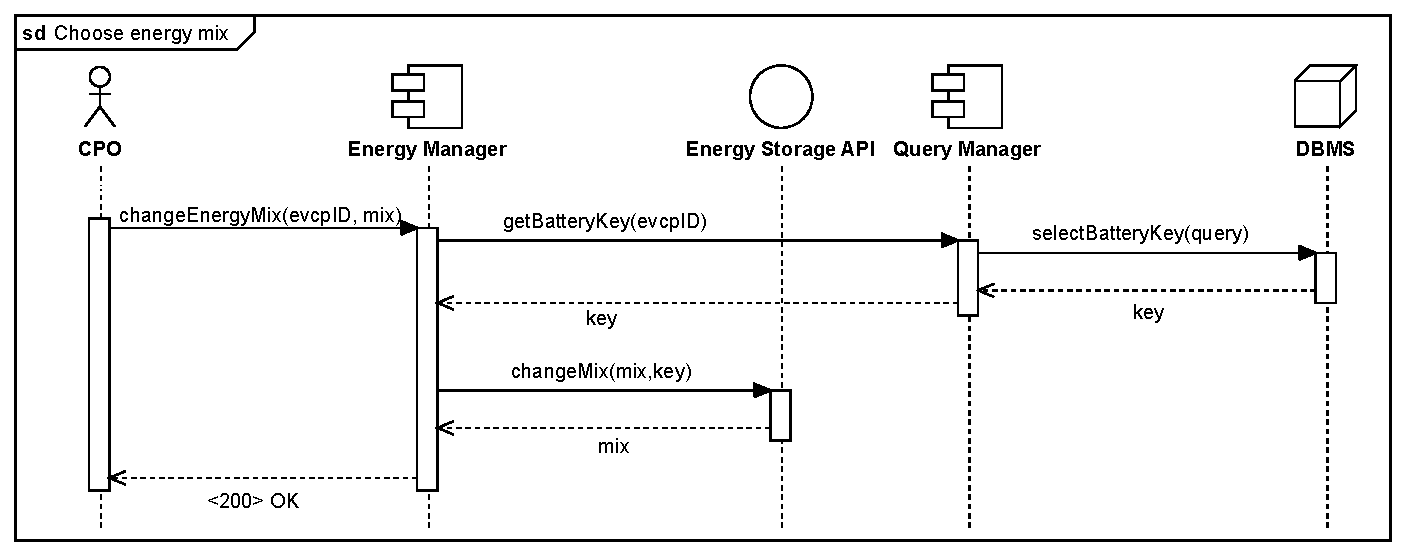
\includegraphics[scale=0.55]{src/runtimeView/CPMS_energyMix.pdf}
              \caption{Choose energy Mix}
          \end{figure}
    \item \textbf{Choose DSO} : The following diagram represents the workflow when the CPO chooses DSO.\\
          \\ The CPO chooses DSO interacting with the Energy Manager. The Energy Manager interacts with the Query Manager obtaining the Commitment Date of the actual contract.
          If the Commitment date is not reached yet, the Energy Manager responds that the request is not valid.
          Otherwise, the Energy Manager interacts with the Energy Storage API obtaining a contract. Then the Energy Manager sends an ack to the CPO and interacts with the
          Query Manager to store the new contract.
          \begin{figure}[H]
              \centering
              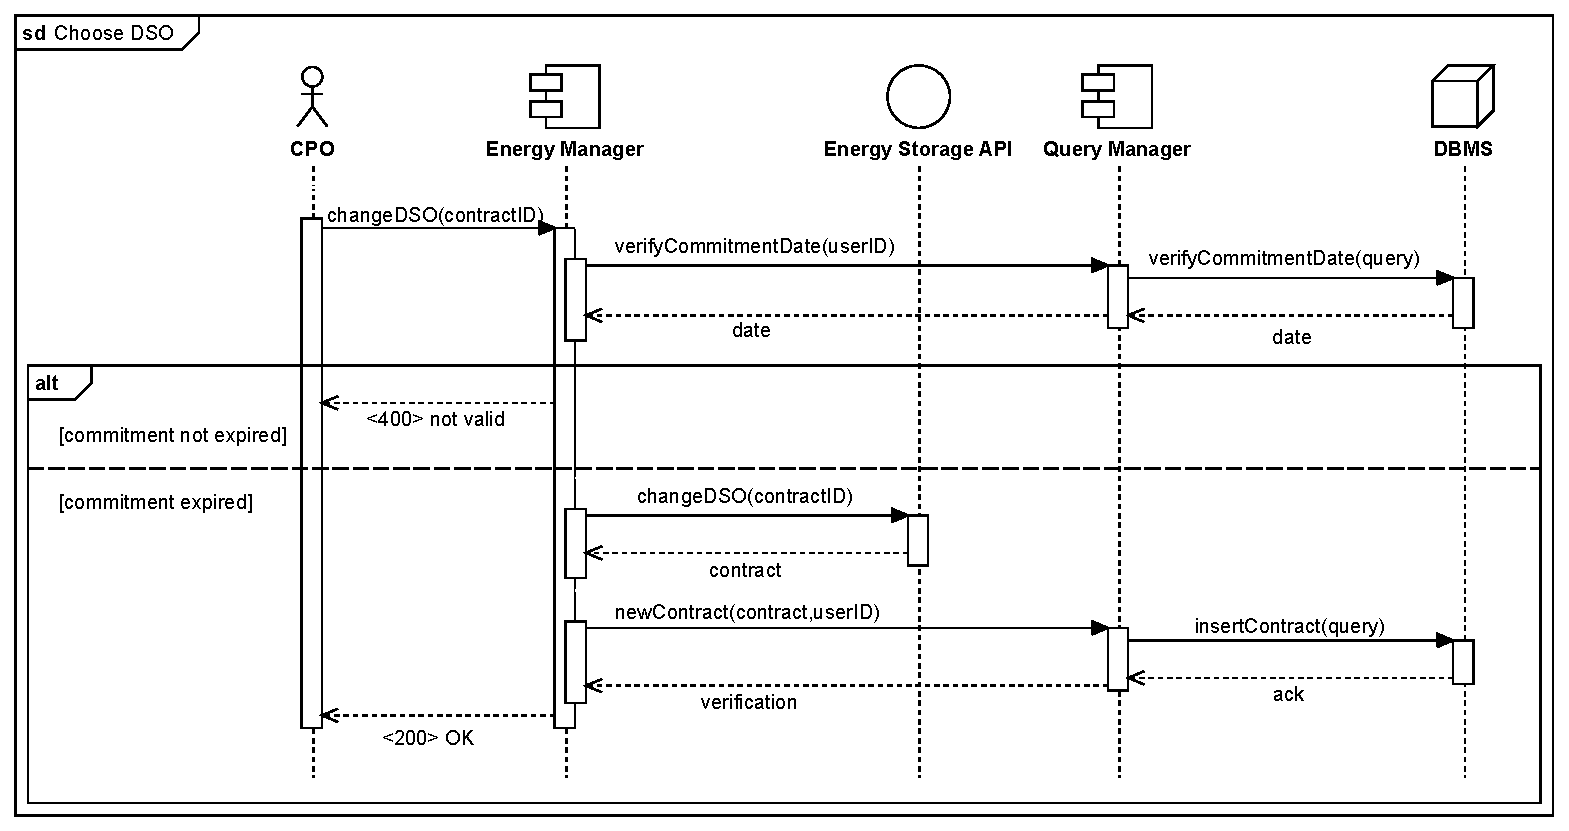
\includegraphics[scale=0.55]{src/runtimeView/CPMS_chooseDSO.pdf}
              \caption{Choose DSO}
          \end{figure}



\end{itemize}

\subsection{Component interfaces}
Details for each interface (name, signature, returned objects)
\subsubsection{REST Endpoints}
\renewcommand{\labelitemii}{}
\renewcommand{\labelitemiii}{-}
\begin{itemize}
    \item \texttt{/api/search/<latitude|longitude>}
          \begin{itemize}
              \item Maps: \texttt{NomeMetodoMappato}
              \item Type: TipoAPI(GET,POST)
              \item URL Parameters:
                    \begin{itemize}
                        \item \texttt{<latitude|longitude>} - GPS Location, needed to find CPs nearby a certain location.
                    \end{itemize}
              \item Parameters:
                    \begin{itemize}
                        \item \texttt{authToken}
                        \item \texttt{blabla} [string] - description
                        \item \texttt{blabla} [boolean] - description
                        \item \texttt{blabla} [number] - description
                    \end{itemize}
              \item Success:
                    \begin{itemize}
                        \item 200 - OK + Response
                              \begin{lstlisting}
            {
                "cps": [
                    {
                        "id": "<store id>",
                        "name": "<cp name>",
                        "address": "<address>",
                        "open": <boolean>,
                        "distance": <number>,
                    }
                ]
            }
            \end{lstlisting}
                    \end{itemize}
              \item Errors:
                    \begin{itemize}
                        \item 400 - Bad request
                        \item 404 - No store found
                    \end{itemize}
          \end{itemize}
\end{itemize}

\subsection{Architectural Styles and patterns}
Please explain which styles/patterns you used, why, and how

\begin{itemize}
    \item Three layers and Four Tier: what and why?
    \item RESTful: what and why?
    \item Adapter Pattern: The Query Manager component implements the Adapter pattern, as it mediates between the
          business logic and the DBMS services, exposing only a restricted and higher level set of functionalities.
\end{itemize}
\subsection{Other design decisions}
\subsubsection{PWA}
\dots
\subsubsection{Scale-out}
\dots
\subsubsection{Relational Database}
\dots
\subsubsection{The separation of eMSP and CPMSs}